\chapter{Решение практических задач коррекции расчетных моделей} 

В данной главе рассматривается применение разработанных методик для решения практических задач коррекции, освобождения и синтеза. Развиваются подходы, позволяющие моделировать податливость закреплений в условиях эксперимента. 

\section{Коррекция расчетной модели динамически-подобной модели самолёта \mbox{Ту-204}}

Для апробации разработанной методики коррекции на примере реальной конструкции была выбрана динамически-подобная модель (ДПМ) самолёта \mbox{Ту-204}, выполненная по отсечно-балочной схеме \figref{fig:tu-204-experiment}. Габаритные размеры: размах крыла $ 3172 $ мм, длина фюзеляжа $ 3462 $ мм (масштаб моделирования~$ 1 \div 10 $). Масса модели с датчиками и кабелями составила $ 50.5 $ кг.

\begin{figure}[!htb]
	\centerfloat
	\includegraphics[width = 0.85\textwidth]{tu-204-experiment}
	\caption{Общий вид ДПМ на упругой подвеске} \label{fig:tu-204-experiment}	
\end{figure}

Упругие характеристики фюзеляжа и крыла смоделированы лонжеронами, расположенными по оси жёсткости каждого агрегата. Топливо, коммерческая нагрузка, оборудование, носовая и основные опоры имитировались жёсткими сосредоточенными грузами. Аэродинамические обводы выполнены в виде лёгких отсеков. Для проведения экспериментального модального анализа ДПМ была вывешена на упругой подвеске малой жесткости.

Исходя из типа схематизации ДПМ, первоначально было принято решение о создании балочной КЭ-модели. Распределение массы конструкции считалось дискретным, а распределение жесткостных характеристик~---~линейным по длине каждой из балок. При моделировании по представленной схеме особую сложность составило описание жесткостных характеристик узлов сочленения агрегатов планера. Так, по результатам расчета на собственные частоты и формы колебаний, было выяснено, что балочная расчетная модель некорректно описывает динамическое поведение реальной ДПМ, в связи с чем было принято решение отказаться от ее дальнейшего использования в пользу объемной конечно-элементной модели.

Создание трехмерной геометрической модели \figref{fig:tu-204-geometry-full} проводилось по натурной ДПМ. Геометрические модели крыльевых отсеков не создавались, так как они, в силу конструктивного исполнения ДПМ, являются точечными массами для упругого крыла~---~не вносят жесткостей и не соприкасаются между собой при малых амплитудах колебаний. В силу последнего обстоятельства отсеки и хвостовое оперение при создании КЭ-модели также моделировались дискретными массами с инерционными характеристиками, определенными по соответствующим геометрическим моделям~\figref{fig:tu-204-geometry-masses}. 

\begin{figure}[!htb]
	\centerfloat
	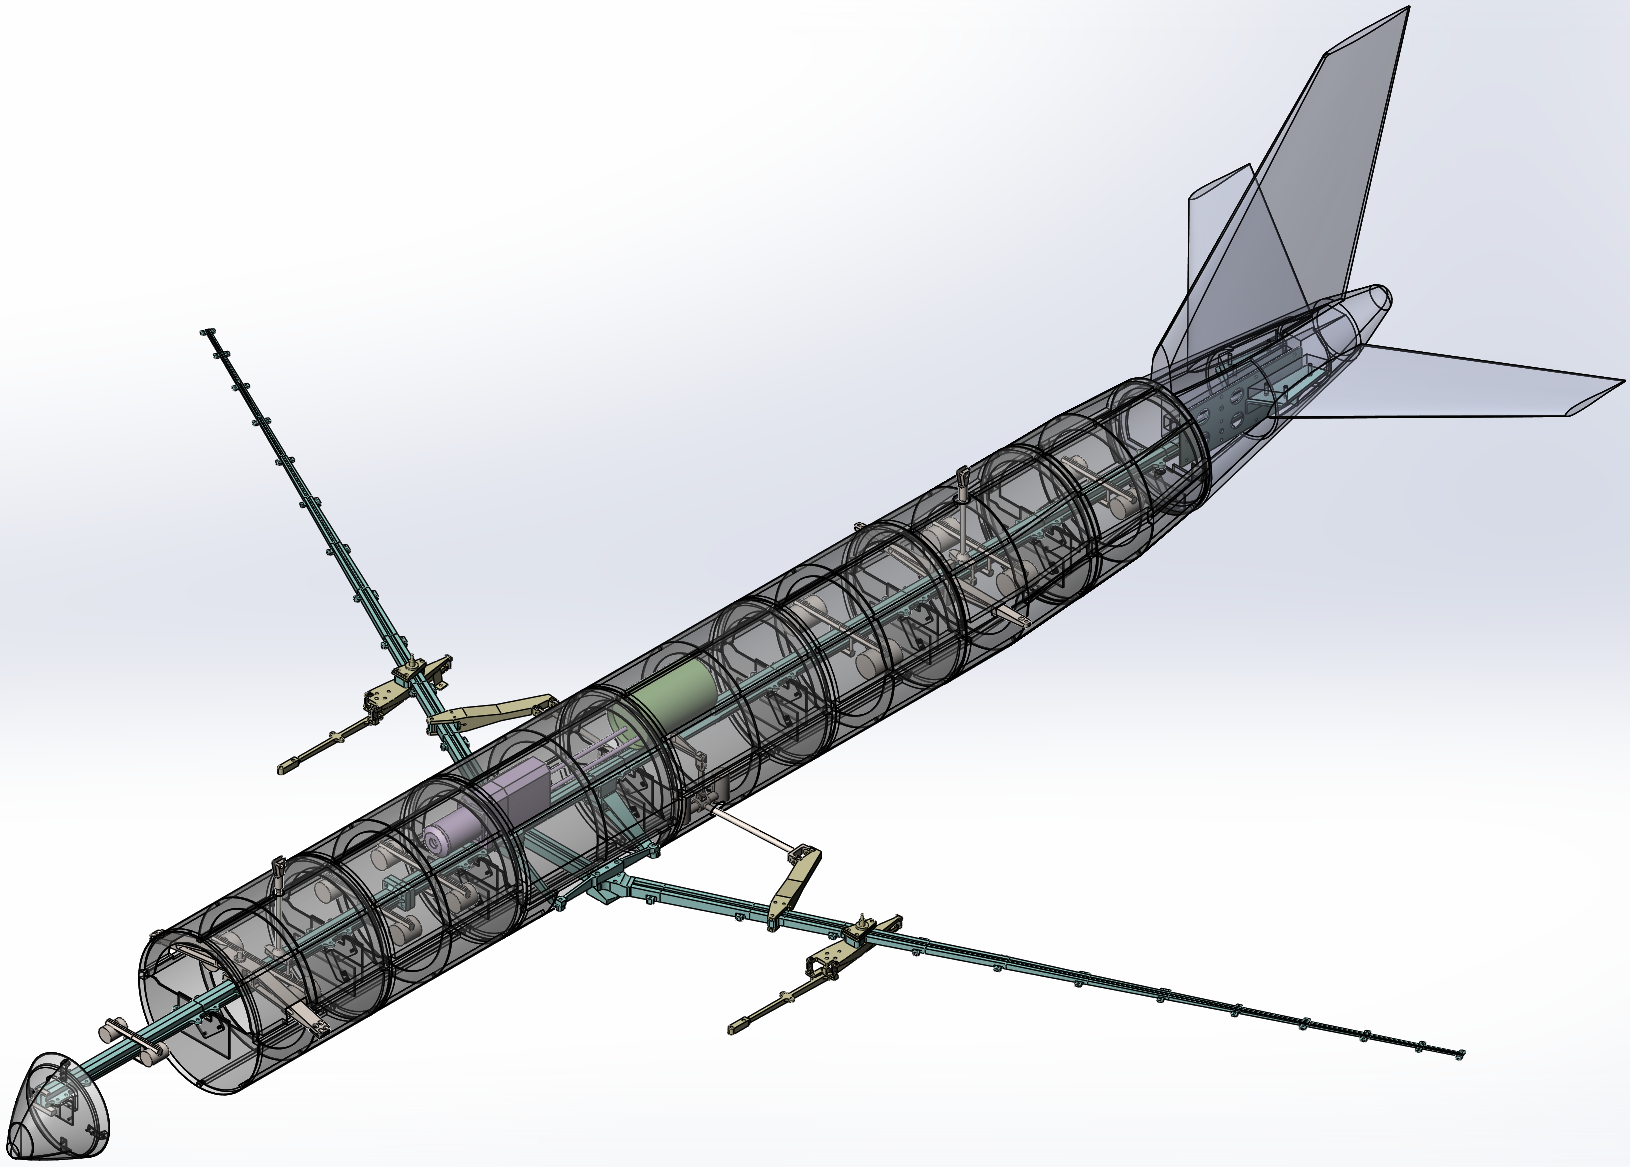
\includegraphics[width = 0.85\textwidth]{tu-204-geometry-full}
	\caption{Геометрическая модель ДПМ} \label{fig:tu-204-geometry-full}
\end{figure}

\begin{figure}[!htb]
	\centerfloat
	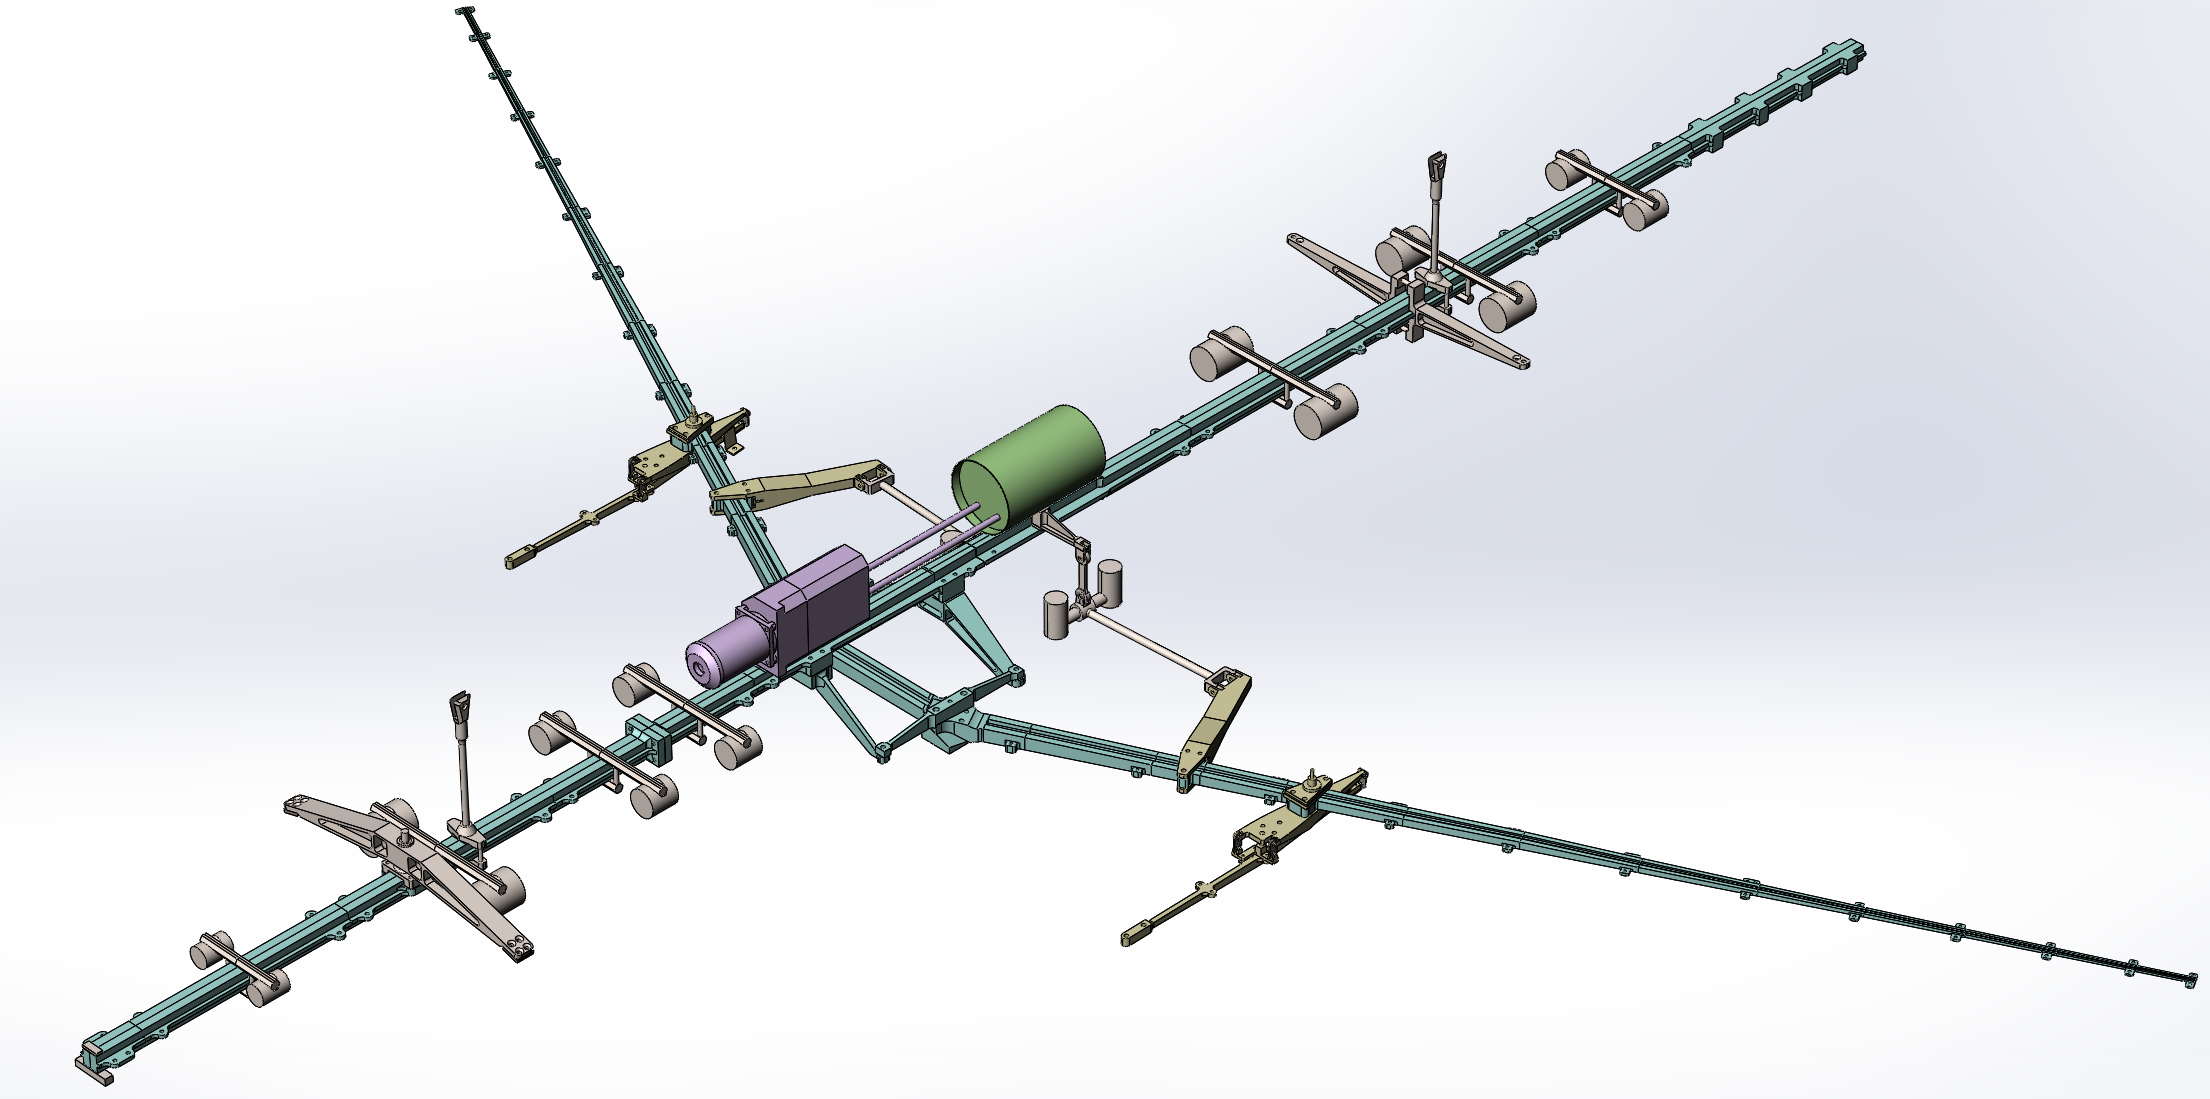
\includegraphics[width = 0.85\textwidth]{tu-204-geometry-masses}
	\caption{Геометрическая модель ДПМ без фюзеляжных отсеков и хвостового оперения} \label{fig:tu-204-geometry-masses}
\end{figure}

Для достоверного определения инерционных характеристик исключенных из модели агрегатов их массы были скорректированы по результатам взвешивания. Аналогичная процедура была проведена для моделирования коммерческой загрузки дискретными массами. Отметим, что было достигнуто удовлетворительное согласование масс лонжерона крыла и фюзеляжа расчетной модели с данными технической документации ДПМ.

По выгруженной из \name{Solidworks} геометрической модели была создана КЭ-модель \name{Ansys}~\figref{fig:tu-204-mesh} с числом степеней свободы~---~$ 752 $ тысячи. Стандартные инструменты графической оболочки конечно-элементного модуля \name{Ansys Workbench} предусматривают лишь возможность создания дискретных масс без учета центробежных моментов инерции. Поэтому был разработан скрипт на языке \name{Ansys APDL} для расширения существующего инструментария: моделирование дискретных масс по заданным матрицам инерции. 

Расположение дискретных масс, моделирующих агрегаты планера и коммерческую загрузку, формировались посредством графического интерфейса \name{Ansys Workbench} и установления их именного соответствия с инерционными характеристиками (масса, положение и матрица инерции) в текстовом файле. В ходе расчета разработанным скриптом создаются дополнительные массовые элементы \name{Matrix27}, которые присоединяются жесткими невесомыми балками к узлам, принадлежащим выбранным областям. 

\begin{figure}[H]
	\centerfloat
	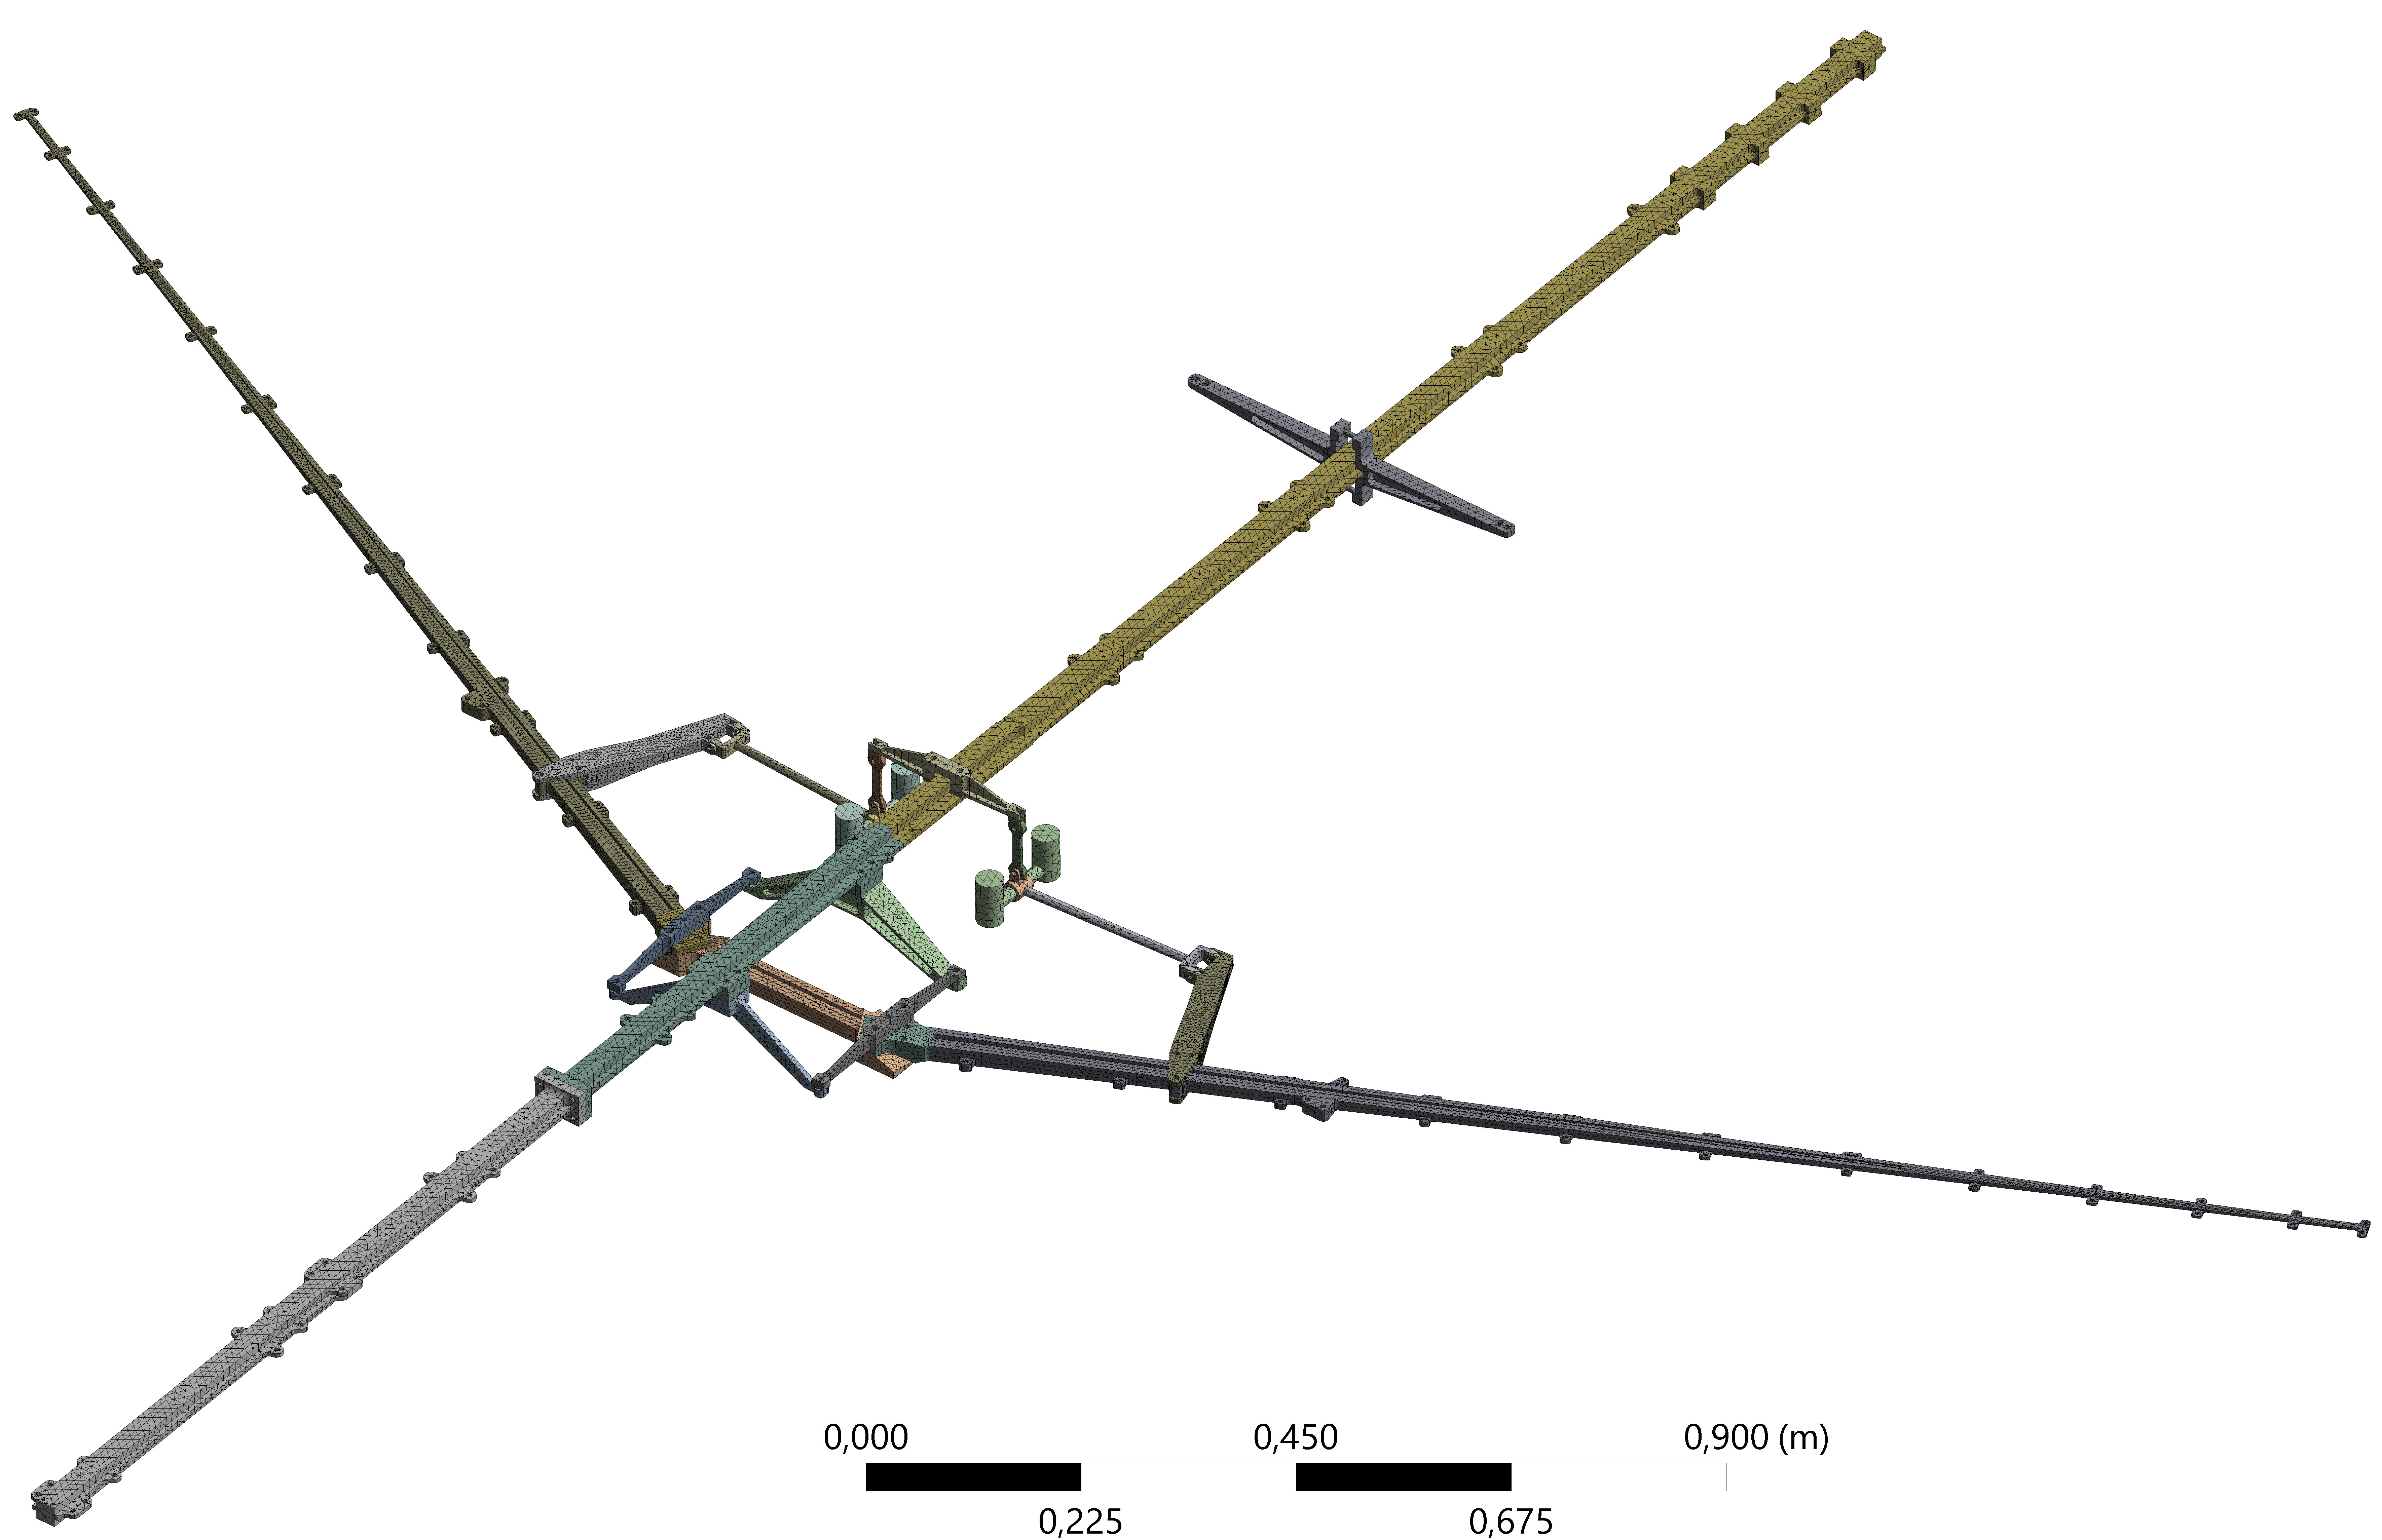
\includegraphics[width = 0.85\textwidth]{tu-204-mesh}
	\caption{Конечно-элементная модель ДПМ} \label{fig:tu-204-mesh}
\end{figure}

Дискретизация конечно-элементной модели выбрана из условия корректного описания геометрических особенностей узлов сочленения и навески агрегатов планера.

Коррекция КЭ-модели проводилась по шести наборам экспериментально определенных частот собственных колебаний:
\begin{enumerate}
	\item по 7 тону~---~симметричный изгиб крыла I тона~(СИКр1);
	\item с 7 по 8 тон~---~СИКр1, антисимметричный изгиб крыла I тона~(АСИКр1);
	\item с 7 по 9 тон~---~СИКр1, АСИКр1, горизонтальный изгиб фюзеляжа I тона~(ГИФ1);
	\item с 7 по 10 тон~---~СИКр1, АСИКр1, ГИФ1, вертикальный изгиб фюзеляжа I тона (ВИФ1);
	\item с 7 по 10 и 12 тону~---~СИКр1, АСИКр1, ГИФ1, ВИФ1, симметричный изгиб крыла II тона (СИКр2);
	\item с 7 по 10, 12 и 15 тонам~---~СИКр1, АСИКр1, ГИФ1, ВИФ1, СИКр2, вертикальный изгиб фюзеляжа II тона~(ВИФ2).
\end{enumerate}

Итерационный процесс коррекции по предложенному алгоритму считался завершенным при достижении
целевых значений частот с точностью 0.0001 \%. Результаты коррекции сведены в таблице \ref{tab:updatingTu204}. 

\begin{longtblr}[
	caption = {Результаты коррекции ДПМ самолёта \mbox{Ту-204}}, 
	label = {tab:updatingTu204}
]{
	colspec = {|c|c|c|c|X[c]|X[c]|X[c]|X[c]|X[c]|X[c]|}, 
	hlines
}
   	\SetCell[r = 3]{c} Тон & \SetCell[c = 2]{c} Частоты, Гц && \SetCell[c = 7]{c} Погрешность до и после коррекции, \%  \\
   	& \SetCell[r = 2]{c} Эксперимент & \SetCell[r = 2]{c} {Исходная \\ модель} & \SetCell[r = 2]{c} До & \SetCell[c = 6]{c} После \\ 
   	& & & & 1 & 2 & 3 & 4 & 5 & 6 \\ \hline
	СИКр1 & 3.44 & 3.49 & 1.5 & 0.0 & 0.0 & 0.0 & 0.0 & 0.0 & 0.0 \\
	АСИКр1 & 4.87 & 4.96 & 1.7 & -0.6 & 0.0 & 0.0 & 0.0 & 0.0 & 0.0 \\
	ГИФ1 & 5.44 & 5.73 & 5.3 & 4.7 & 4.7 & 0.0 & 0.0 & 0.0 & 0.0 \\ 
	ВИФ1 & 5.73 & 5.97 & 4.2 & 3.5 & 3.3 & 2.6 & 0.0 & 0.0 & 0.0 \\
	СИКр2 & 9.30 & 9.13 & -1.8 & -4.4 & -3.2 & -3.9 & -4.4 & 0.0 & 0.0 \\
	ВИФ2 & 14.18 & 14.77 & 4.2 & 3.7 & 3.8 & 3.4 & 2.0 & 3.3 & 0.0 \\
\end{longtblr}

Распределения изменений узловых жестокостей по всем линейным степеням свободы КЭ-модели до и после каждой из коррекций
приведены на рисунке~\ref{fig:tu-204-coeffs}.

\def\sfTu204Dist{0.4\textwidth}

\begin{figure}[H]
	\centering
	\begin{subfigure}[b]{\sfTu204Dist}
		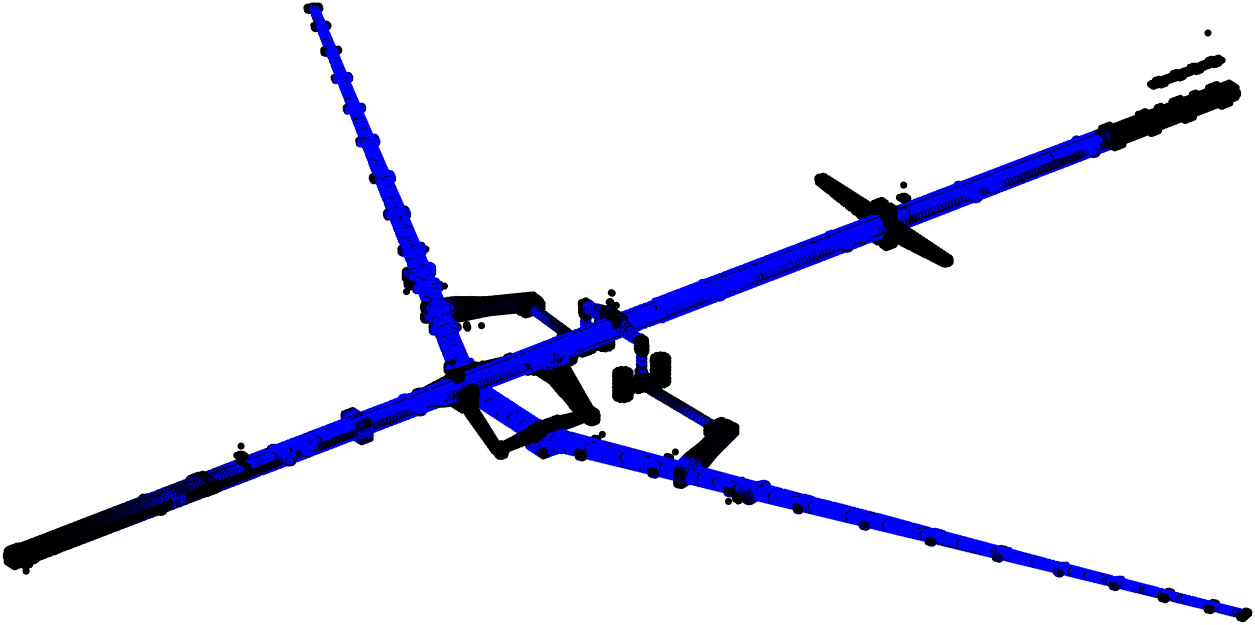
\includegraphics[width = \textwidth]{tu-204-coeffs-1}
		\caption{} \label{subfig:tu-204-coeffs-1}
	\end{subfigure}
	\begin{subfigure}[b]{\sfTu204Dist}
		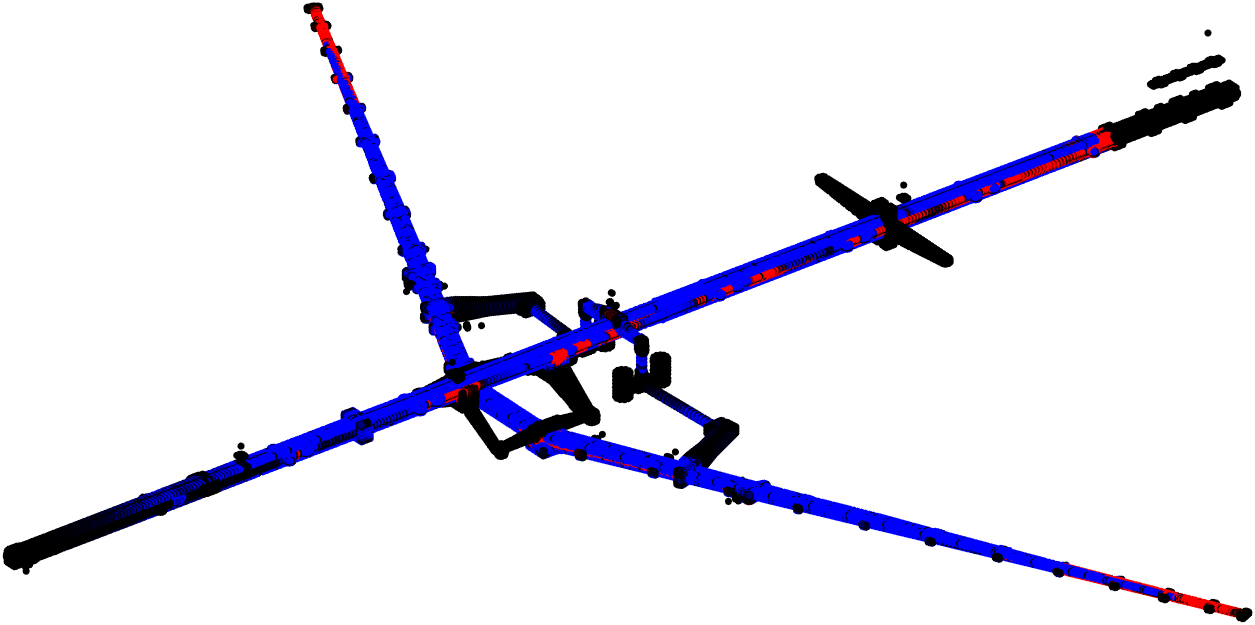
\includegraphics[width = \textwidth]{tu-204-coeffs-2}
		\caption{}
	\end{subfigure}
	\begin{subfigure}[b]{\sfTu204Dist}
		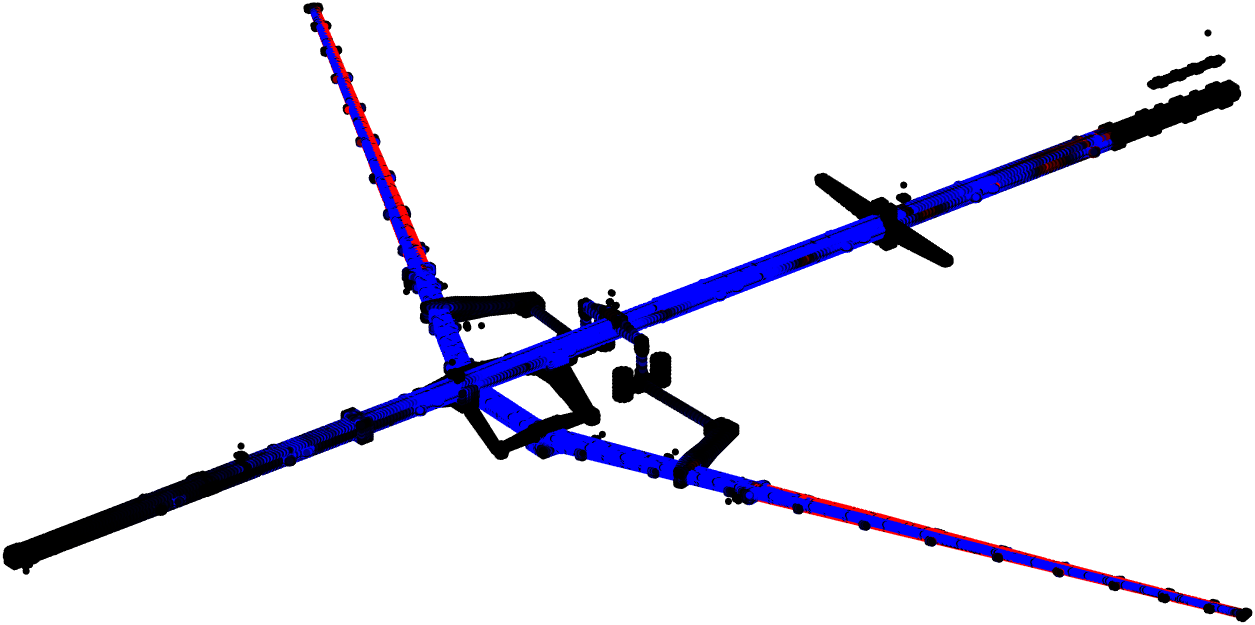
\includegraphics[width = \textwidth]{tu-204-coeffs-3}
		\caption{}
	\end{subfigure}	
	\begin{subfigure}[b]{\sfTu204Dist}
		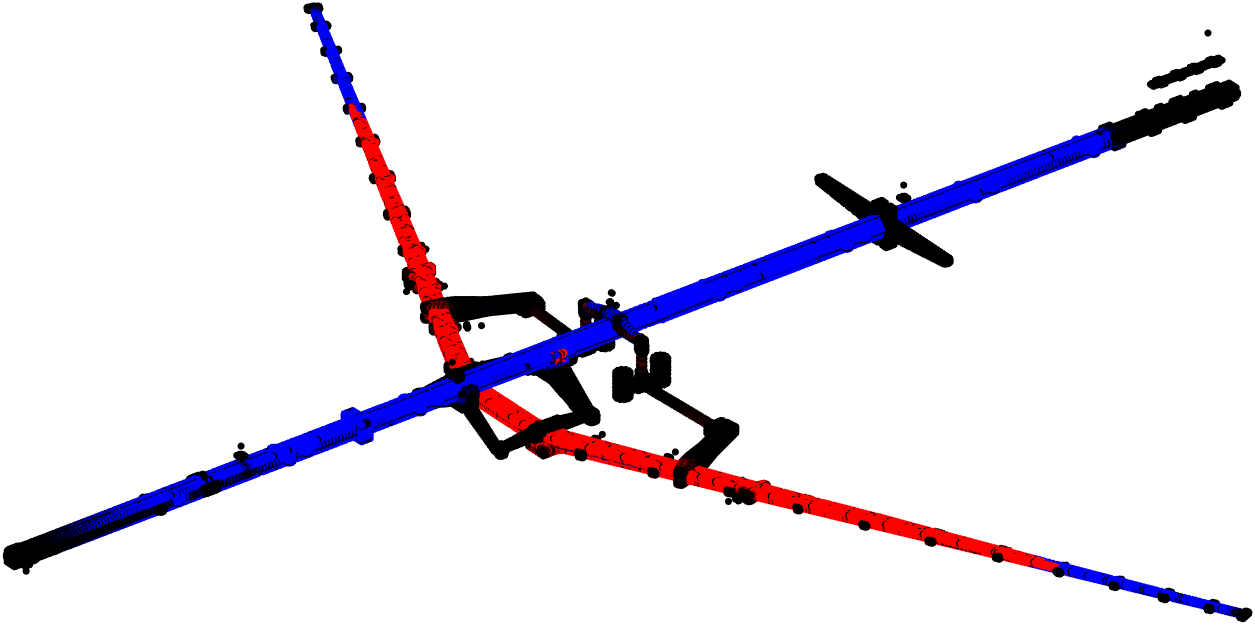
\includegraphics[width = \textwidth]{tu-204-coeffs-4}
		\caption{}
	\end{subfigure}	
	\begin{subfigure}[b]{\sfTu204Dist}
		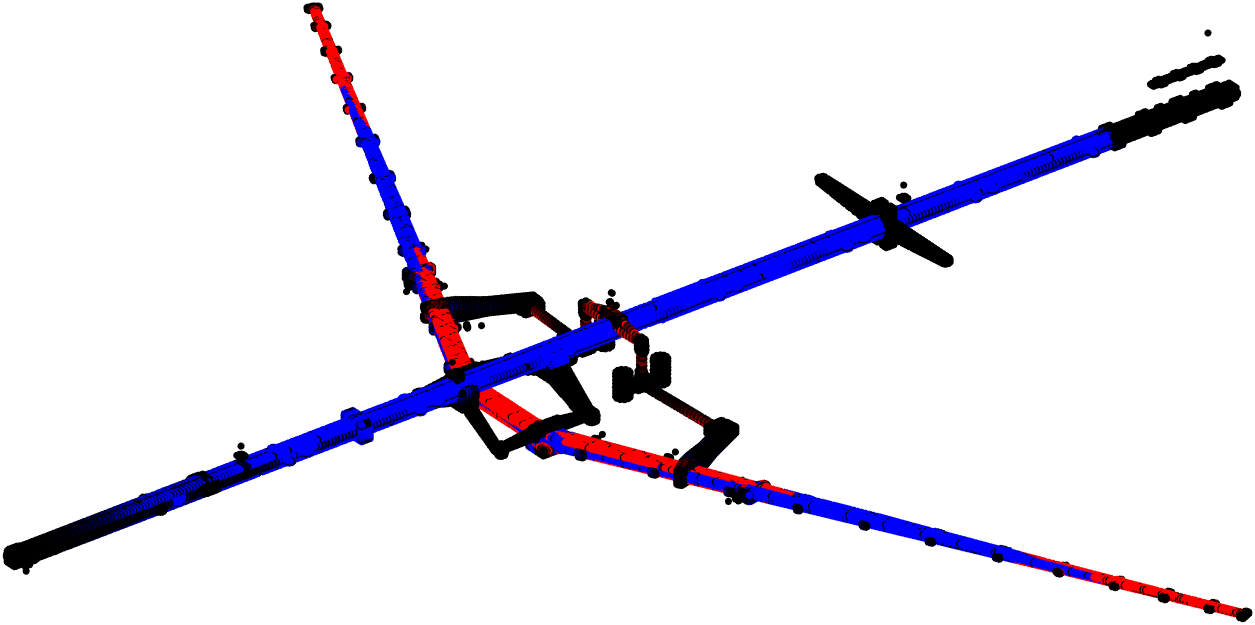
\includegraphics[width = \textwidth]{tu-204-coeffs-5}
		\caption{}
	\end{subfigure}
	\begin{subfigure}[b]{\sfTu204Dist}
		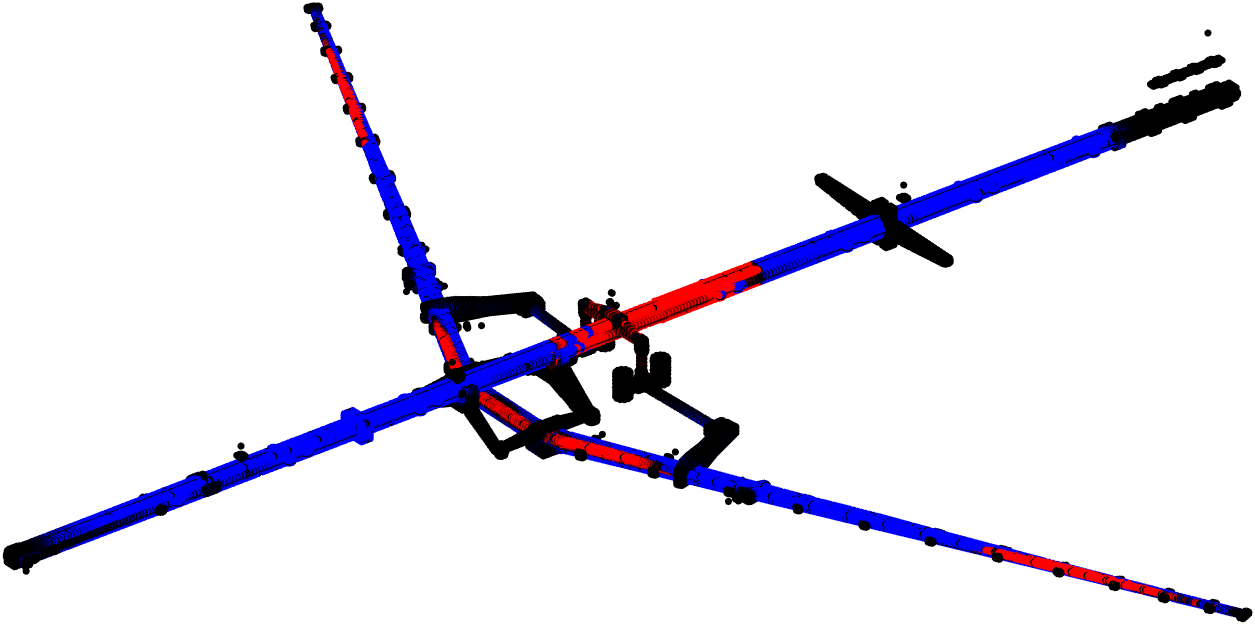
\includegraphics[width = \textwidth]{tu-204-coeffs-6}
		\caption{} \label{subfig:tu-204-coeffs-6}
	\end{subfigure}
	\caption{Распределения изменений узловых жесткостей при коррекции по наборам целевых частот от 1 до 6 (а~--~е)} \label{fig:tu-204-coeffs}
\end{figure}

Синяя цветовая гамма на рисунке соответствует областям понижения исходной жесткости (корректирующая КЭ-модель имеет отрицательную жесткость в этих областях), а красная~---~областям повышения исходной жесткости. Черному цвету соответствуют области, жесткость которых в ходе коррекции осталась неизменной.

Заметим, что коррекция по одному тону (набор 1) приводит к снижению жесткости практически во всех областях~\figref{subfig:tu-204-coeffs-1} с измененной жесткостью. Добавление в набор других тонов приводит к появлению областей с положительным изменением жесткости в узлах (рисунки \ref{subfig:tu-204-coeffs-1}~--~\ref{subfig:tu-204-coeffs-6}). При этом для каждого набора распределение корректирующих жесткостей уникально.

Вследствие изменения упругости корректируемой модели происходит изменение частот и форм колебаний. Нормированные к массе формы колебаний до (серым цветом) и после коррекции (зеленым цветом) по шестому набору частот приведены на рисунке \ref{fig:tu-204-modes}. Из рисунка видно, что формы колебаний до и после коррекции хорошо коррелируют между собой~---~разница между формами колебаний по MAC-критерию до и после коррекции составила: $ 0.02 $, $ 1.12 $, $ 1.74 $, $ 0.87 $, $ 0.18 $ и $ 4.09 $\,\% соответственно.

\def\sfTu204Mode{0.32\textwidth}

\begin{figure}[H]
	\centering
	\begin{subfigure}[b]{\sfTu204Mode}
		\centering
		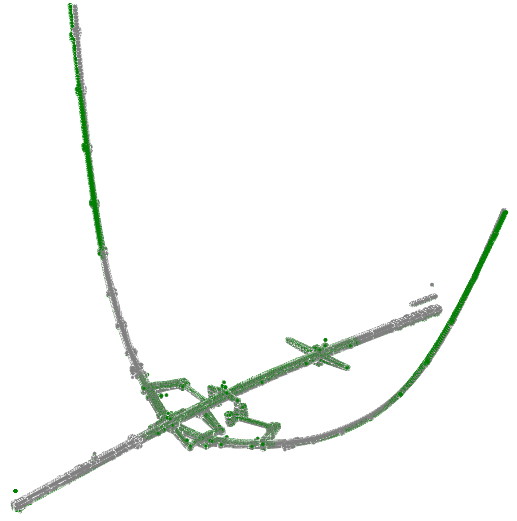
\includegraphics[width = \textwidth]{tu-204-mode-1}
		\caption{СИКр1} 
	\end{subfigure}
	\begin{subfigure}[b]{\sfTu204Mode}
		\centering
		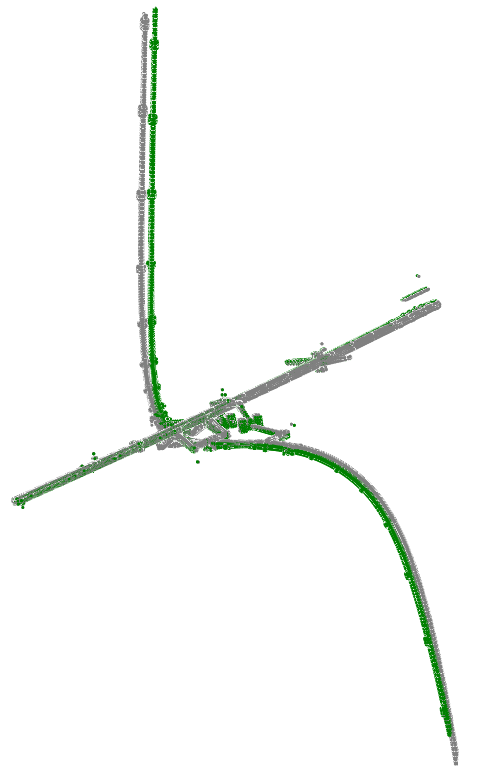
\includegraphics[width = 0.65\textwidth]{tu-204-mode-2}
		\caption{АСИКр1}
	\end{subfigure}
	\begin{subfigure}[b]{\sfTu204Mode}
		\centering
		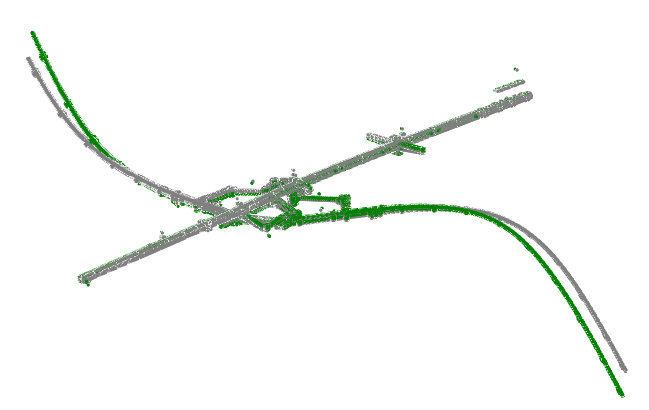
\includegraphics[width = \textwidth]{tu-204-mode-3}
		\caption{ГИФ1}
	\end{subfigure}	
	\begin{subfigure}[b]{\sfTu204Mode}
		\centering
		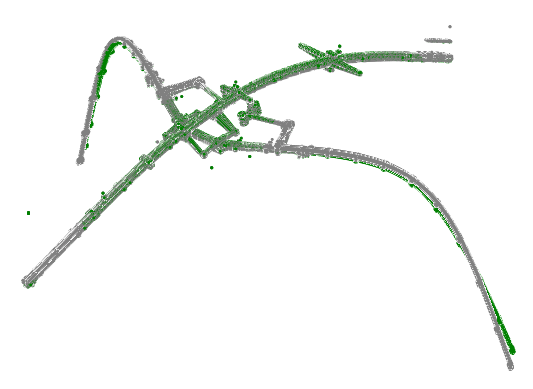
\includegraphics[width = \textwidth]{tu-204-mode-4}
		\caption{ВИФ1}
	\end{subfigure}	
	\begin{subfigure}[b]{\sfTu204Mode}
		\centering
		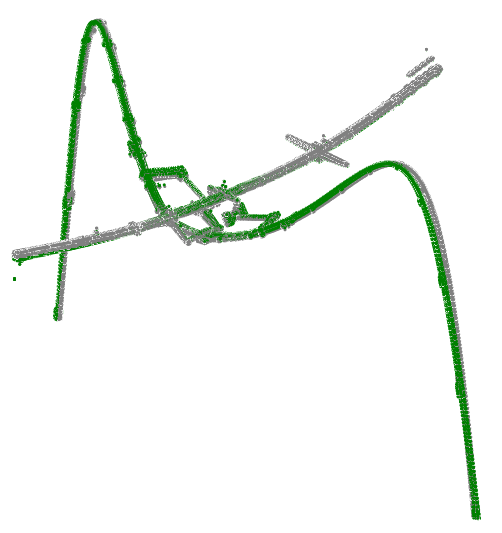
\includegraphics[width = 0.7\textwidth]{tu-204-mode-5}
		\caption{СИКр2}
	\end{subfigure}
	\begin{subfigure}[b]{\sfTu204Mode}
		\centering
		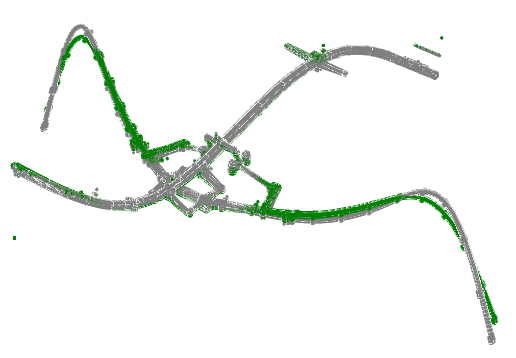
\includegraphics[width = \textwidth]{tu-204-mode-6}
		\caption{ВИФ2} 
	\end{subfigure}
	\caption{Формы колебаний ДПМ до и после коррекции} \label{fig:tu-204-modes}
\end{figure}

\section{Синтез имитационной модели каркаса зонтичной антенны космического аппарата} \label{struct:synthesisApprobation}

С целью апробации методики синтеза была выбрана имитационная модель каркаса зонтичной антенны~\figref{fig:simsat-assembly}. Каркас выполнен из профилированных стальных труб и плоских стальных накладок. Конструктивно модель состоит из зонтичного каркаса и штанги, элементы скреплены болтами. Габаритные размеры показаны на рисунке~\ref{fig:simsat-dimensions}. Масса каркаса $ 73 $ кг, штанги~---~$ 22 $ кг.

\begin{figure}[!htb]
	\centerfloat
	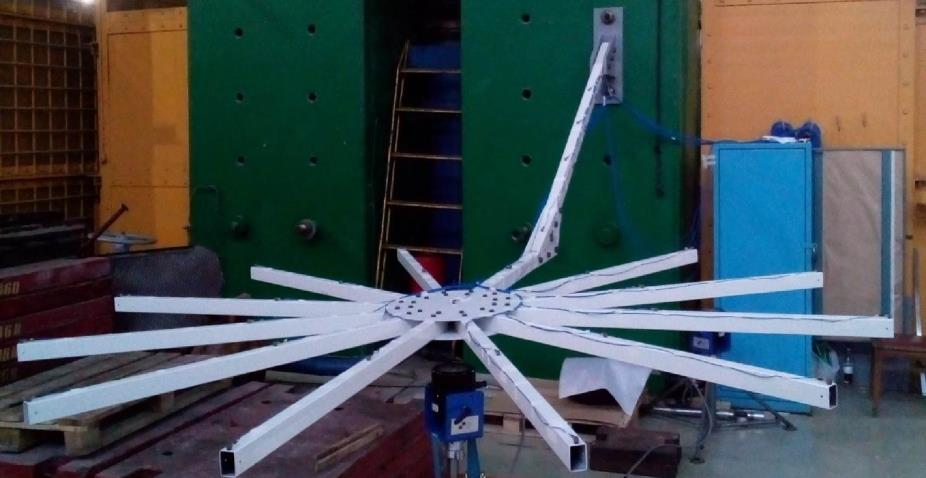
\includegraphics[width = 0.75\linewidth]{simsat-assembly}
	\caption{Общий вид имитационной модели каркаса зонтичной антенны} \label{fig:simsat-assembly}
\end{figure}

\begin{figure}[H]
	\centerfloat
	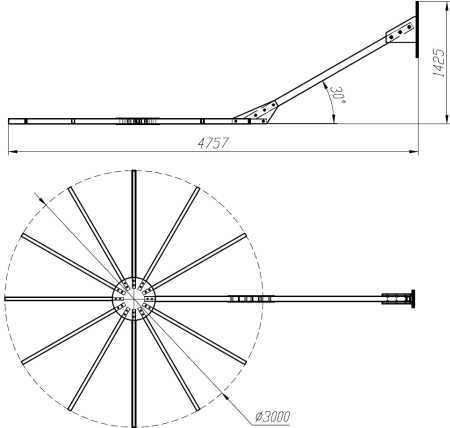
\includegraphics[width = 0.65\linewidth]{simsat-dimensions}
	\caption{Габаритные размеры модели каркаса зонтичной антенны} \label{fig:simsat-dimensions}
\end{figure}

\subsection{Модальные испытания}

В соответствии с предлагаемым расчетно-экспериментальным методом, конструкция разделена на две составные части \figref{fig:simsat-parts}: зонтичный каркас и штангу, для каждой из которых проведен экспериментальный модальный анализ.

\begin{figure}[!htb]
	\centering
	\begin{subfigure}[t]{0.48\textwidth}
		\centering
		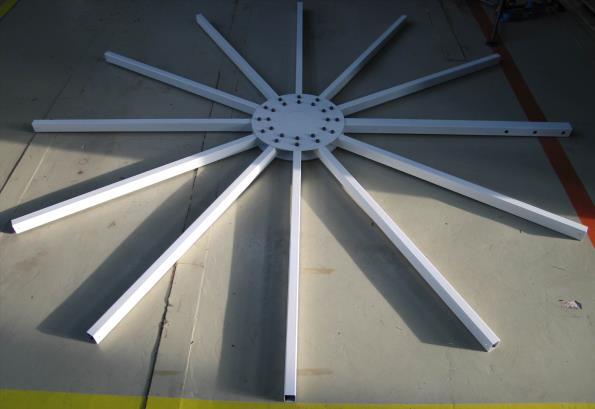
\includegraphics[width = \textwidth]{simsat-antenna}
		\caption{Зонтичный каркас}
	\end{subfigure}
	\hfill
	\begin{subfigure}[t]{0.48\textwidth}
		\centering
		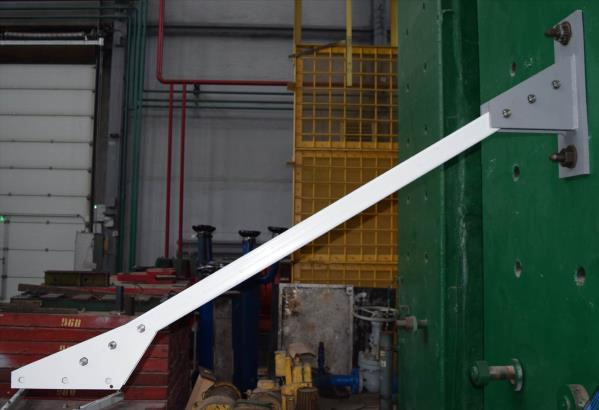
\includegraphics[width = \textwidth]{simsat-handle}
		\caption{Штанга}
	\end{subfigure}	
	\caption{Составные части модели каркаса зонтичной антенны} \label{fig:simsat-parts}
\end{figure}

Для управления возбуждением и измерением колебаний использовалась многоканальная система \name{LMS SCADAS Lab} \figref{fig:lms-scadas}, включавшая в себя персональный компьютер со специализированным программным обеспечением \name{LMS TestLab}. Система измерений состояла из $ 19 $ блоков восьмиканальных измерительных усилителей стандарта \name{IEPE} ($ 152 $ входных канала). Управление возбуждением колебаний осуществлялось шестиканальным генератором сигналов, позволяющим независимое варьирование амплитудой и фазой сигнала каждого канала. Возбуждение колебаний объекта испытаний осуществлялось электродинамическими силовозбудителями (ЭДСВ) \name{2060E} с усилителями мощности модели \name{2050E09}  производства компании \name{TMS} \figref{fig:simsat-handle-test}. Максимальное номинальное усилие, развиваемое ЭДСВ~---~$ 267 $ Н. Измерение сил проводилось датчиками динамической силы модели \name{208C02} производства компании \name{PCB Piezotronics}. Возбуждающие силы прикладывались к элементам конструкции через стержни с малой изгибной жёсткостью. Виброускорения объекта испытаний измерялись в контрольных точках конструкции акселерометрами стандарта \name{IEPE} модели \name{333B30} производства компании \name{PCB Piezotronics} и модели \name{АР2043-100} производства \name{Глобалтест} \figref{fig:simsat-handle-test}. Акселерометры крепились на поверхность объекта с помощью восковой мастики.

\begin{figure}[!htb]
	\centerfloat
	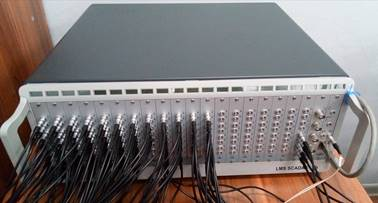
\includegraphics[width = 0.6\linewidth]{lms-scadas}
	\caption{Система управления испытаниями \name{SCADAS Lab}} \label{fig:lms-scadas}
\end{figure}

\begin{figure}[!htb]
	\centerfloat
	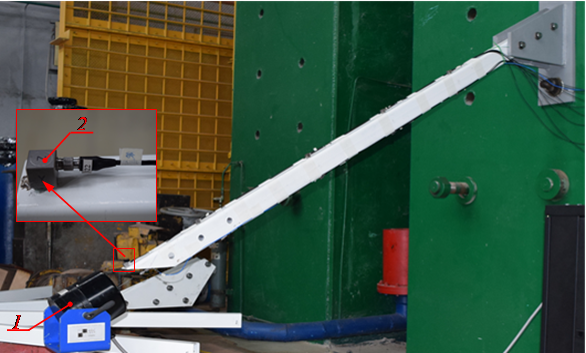
\includegraphics[width = 0.6\linewidth]{simsat-handle-test}
	\caption{Модальные испытания штанги: 1~---~ЭДСВ, 2~---~акселерометр} \label{fig:simsat-handle-test}
\end{figure}

Расчётные исследования скорректированной по результатам испытаний математической модели показали, что узел крепления штанги к силовой колонне имеет недостаточную жёсткость в боковом направлении. Поэтому конструкция кронштейна была изменена \figref{fig:simsat-handle-fixture}. 

\begin{figure}[!htb]
	\centering
	\begin{subfigure}[t]{0.335\textwidth}
		\centering
		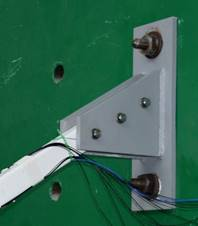
\includegraphics[width = \textwidth]{simsat-handle-fixture-init}
		\caption{Исходный}
	\end{subfigure}
	\qquad
	\begin{subfigure}[t]{0.35\textwidth}
		\centering
		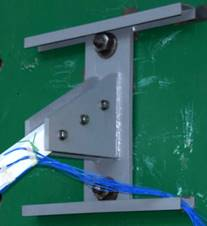
\includegraphics[width = \textwidth]{simsat-handle-fixture-improved}
		\caption{Модернизированный}
	\end{subfigure}	
	\caption{Узел крепления имитационной модели к силовой колонне} \label{fig:simsat-handle-fixture}
\end{figure}

Установлено, что закрепление подконструкций на время испытаний в узлах стыковки приводит к потере информации о степенях свободы этих узлов в скорректированной расчётной модели. Поэтому зонтичный каркас был доработан для обеспечения его крепления в центральной части, а не за одну из спиц. На нижней поверхности каркаса установлена гайка с упорами для фиксации его на жёсткой опоре \figref{fig:simsat-antenna-welded}. Собственная частота низшего тона колебаний составила $ 6.095 $~Гц.

\begin{figure}[!htb]
	\centerfloat
	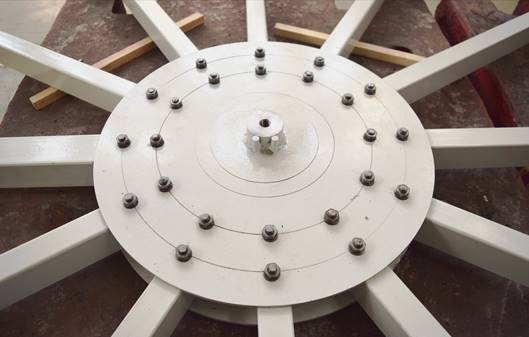
\includegraphics[width = 0.7\linewidth]{simsat-antenna-welded}
	\caption{Узел крепления зонтичного каркаса} \label{fig:simsat-antenna-welded}
\end{figure}

Затем были проведены модальные испытания полностью собранной имитационной модели для проверки результатов коррекции, освобождения и ассемблирования. 

\subsection{Разработка расчетной модели} \label{struct:simsat-model}

Расчетная модель имитационной модели несколько раз уточнялась и претерпевала изменения в связи с отработкой методики ассемблирования и коррекции динамических свойств её составных частей. Прорабатывались такие аспекты, как моделирование узлов стыковки составных частей, моделирование контактного взаимодействия оболочечных элементов при переходе от исходной геометрии к срединным плоскостям. Кроме того, прорабатывались различные варианты крепления штанги к стене из-за невозможности привести динамические параметры модели к параметрам, определенным из эксперимента, что, в итоге, привело к необходимости произвести оценку жесткости крепления штанги к стене. Методика оценки "<жесткости заделки"> описана далее в тексте настоящей работы. Кроме того, проводились исследования с целью определения влияния параметров конечно-элементной сетки на результаты коррекции и последующей виртуальной стыковки моделей составных частей. Каждый из полученных результатов также соотносился с результатами натурных экспериментов. 

После проведенных исследований было принято решение отказаться от контактных элементов и моделировать контактные взаимодействия между срединными плоскостями оболочечными элементами. 

Представленные в настоящей работе результаты по коррекции и стыковке получены по КЭ-модели каркаса зонтичной  антенны с числом степеней свободы~---~$ 252375 $, из которых $ 57852 $~---~штанга, $ 194523 $~---~антенна. На рисунке~\ref{fig:simsat-assembly-mesh} представлена сетка конечных элементов имитационной модели зонтичного каркаса антенны.

\begin{figure}[!htb]
	\centerfloat
	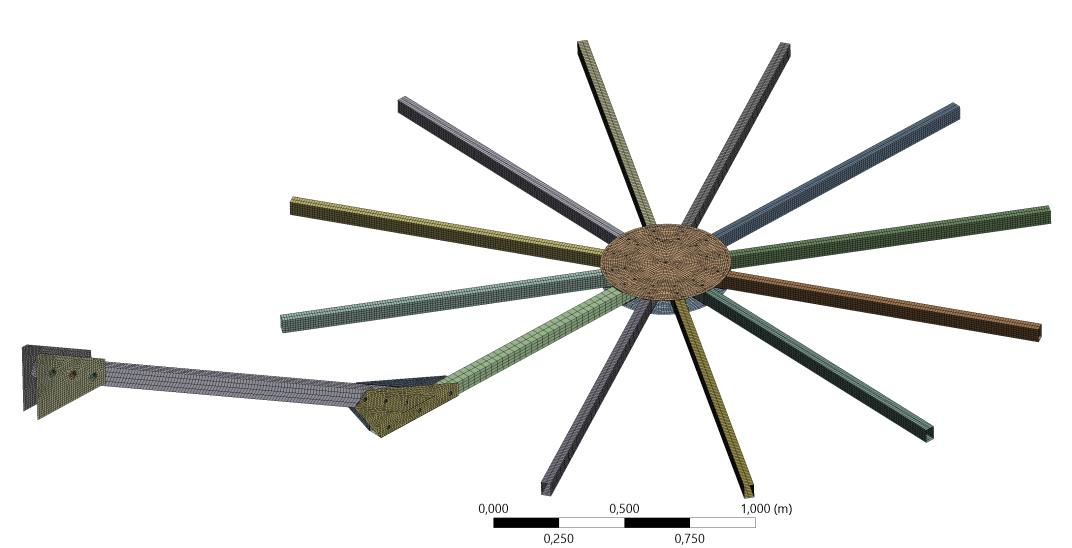
\includegraphics[width = \linewidth]{simsat-assembly-mesh}
	\caption{КЭ-модель имитационной модели в Ansys} \label{fig:simsat-assembly-mesh}
\end{figure}

Идея оценочного расчета <<жесткости заделки>> основана на предположении, что математическая модель конструкции качественно описывает её статическую деформацию, а податливость закрепления вносит поворот конструкции как жесткого целого относительно точки крепления. Для приближенного определения <<жесткости заделки>> рассмотрим следующую расчетную схему \figref{fig:simsat-estimation-scheme}. Видится, что данная схема применима только для протяженных объектов типа штанги.

Приложим силу на конце балки, будем измерять перемещения в двух точках~---~$ A $ и $ B $ \figref{fig:simsat-estimation-scheme}. Представим перемещения точек $ A $ и $ B $~---~$ Y_A, Y_B $ как сумму перемещений от поворота на угол $ \alpha $ как жесткого целого и перемещения $ y_A, y_B $ абсолютно жестко заделанной конструкции под действием приложенной нагрузки. Перемещения $ Y_A, Y_B $ определяются из натурного эксперимента, а перемещения $ y_A, y_B $~---~из виртуального, однако, из-за предполагаемого несоответствия математической модели по количественным показателям, для вывода формулы определения <<жесткости заделки>> будем использовать отношение перемещений, а не их абсолютные значения, предполагая, что математическая модель качественно описывает относительные перемещения конструкции при приложении статической нагрузки.

Положим, что перемещения малы, тогда можно записать следующее соотношение:
\begin{equation}
	\frac{Y_A - \ell_A \sin \alpha}{Y_B - \ell_B \sin \alpha} = \frac{y_A}{y_B}.
	\label{eq:fraction-displacements}
\end{equation}

Из \eqref{eq:fraction-displacements} можно получить выражение для угла:
\begin{equation}
	\alpha = \arcsin \rbrackets{\frac{Y_A - Y_B \frac{y_A}{y_B}}{\ell_A - \ell_B \frac{y_A}{y_B}}}.
	\label{eq:estimated-angle}
\end{equation}

\begin{figure}[!htb]
	\centerfloat
	\begin{tikzpicture}[scale = 1, > = stealth]
		% Задание переменных
		\pgfmathsetmacro{\L}{12} 
		\pgfmathsetmacro{\angle}{20}
		\pgfmathsetmacro{\RPoint}{0.1}
		% Стили
		\tikzstyle{lineStart} = [fill = blue!15]
		\tikzstyle{point} = [draw = black!50, fill = black!20, thick, inner sep = 0pt, minimum size = 2mm]
		\tikzstyle{basedim} = [<->, very thick]
		\tikzstyle{curlydim} = [decorate, very thick]
		\tikzstyle{beamdim} = [curlydim, decoration = {calligraphic brace, mirror, raise = 5pt, amplitude = 6pt}]
		% Недеформированная балка
		\begin{scope}[dashed, thin, color = black, scale = 2]
			\point{s}{0}{0}; \support{3}{s}[-90];
		\end{scope}
		\draw[very thick, black] (0, 0) coordinate (orig) -- (\L, 0) coordinate (endInit);
		% Деформированная балка
		\begin{scope}[scale = 2, blue]
			\point{sr}{0}{0}; \support{3}{sr}[-90-\angle];
		\end{scope}
		\draw[ultra thick, blue] (0, 0) .. controls (3, -0.35) and (6, -1) .. (11.3, -2.5);
		% Повернутая балка
		\draw[thick, black] (0, 0) -- (11.75, -1.3) coordinate (endRot);
		% Точки
		\draw[point] (9, 0) circle (\RPoint) node (B) [above right = 2mm] {$ B $};
		\draw[point] (11, 0) circle (\RPoint) node (A) [above right = 2mm] {$ A $};
		% Размеры
			% A
		\draw[basedim] (10.5, -2.2) -- (10.7, -1.25) node [midway, left = 0.5mm] {$ y_A $};
		\draw[beamdim] (10.5, -2.2) -- (11, 0) node [midway, above right, xshift = 3.5mm, yshift = -2mm] {$ Y_A $};
			% B
		\draw[basedim] (8.6, -1.75) -- (8.8, -1) node [midway, left = 0.5mm, yshift = 0.1mm] {$ y_B $};
		\draw[beamdim] (8.6, -1.75) -- (9, 0) node [midway, above right, xshift = 3.5mm, yshift = -2mm] {$ Y_B $};
			% До точек
		\draw[curlydim, decoration = {calligraphic brace, raise = 3pt, amplitude = 15pt}] (0, 0) -- (9, 0) node [midway, above = 3mm, xshift = 5mm] {$ l_B $};
		\draw[curlydim, decoration = {calligraphic brace, raise = 3pt, amplitude = 45pt}] (0, 0) -- (11, 0) node [midway, above = 12mm, xshift = 6mm, yshift = 0mm] {$ l_A $};
		% Нагрузка
		\draw[line width = 3pt, ->] (\L, 2.5) -- (\L, 0) node [midway, right] { $ P $ };
		\draw[basedim] (0, 2.25) --++ (\L, 0) node [midway, above = 0.5mm] {$ l_P $};
		\draw (0, 0) -- (0, 2.5);
		% Угол
		\draw pic [draw, <-, very thick, angle radius = 6cm] {angle = endRot--orig--endInit};
		\draw (6.3, -0.35) node {$ \alpha $};
		\draw (0, 1) coordinate (startSup) -- (orig) -- (0.75, 2) coordinate (endSup)
        	pic [draw, <-, very thick, angle radius = 1.5cm] {angle = endSup--orig--startSup};
        \draw (0.3, 1.75) node {$ \alpha $};
	\end{tikzpicture}
	\caption{Расчетная схема <<жесткости заделки>>} \label{fig:simsat-estimation-scheme}
\end{figure}

С помощью выражения для угла \eqref{eq:estimated-angle} можно рассчитать <<жесткость заделки>>, зная расстояние до приложенной силы $ \ell_P $, но в зависимости от принятой математической модели упругой заделки целесообразно выражать конкретные параметры. Примем модель <<упругой заделки>> в виде четырехугольной абсолютно жесткой невесомой пластины с четырьмя одинаковыми пружинами \figref{fig:simsat-fixture-scheme}, которая может поворачиваться только в горизонтальном и вертикальном направлениях. Такой шарнир реализуется запрещением всех перемещений центральной точки пластины~--~центра поворота и запрещением перемещений из плоскости всем остальным точкам пластины. Таким образом, пластина может только поворачиваться в двух плоскостях (при условии малости перемещений).

\begin{figure}[H]
	\centerfloat
	\begin{tikzpicture}[scale = 1.1, isometric]
		% Задание переменных
		\pgfmathsetmacro{\width}{8}
		\pgfmathsetmacro{\height}{5}
		\pgfmathsetmacro{\length}{3}
		\pgfmathsetmacro{\hWall}{2}
		\pgfmathsetmacro{\dWall}{0.5}
		\pgfmathsetmacro{\hFixS}{2}
		\pgfmathsetmacro{\hFixE}{1}
		\pgfmathsetmacro{\wFix}{2.5}
		\pgfmathsetmacro{\sD}{2}
		\pgfmathsetmacro{\eD}{0.4}
		\pgfmathsetmacro{\op}{0.95}
		% Стили
		\tikzstyle{plate} = [ultra thick, fill = blue!30, draw = black, opacity = \op]
		\tikzstyle{fixture} = [ultra thick, fill = green!10, draw = black, opacity = \op]
		\tikzstyle{spring} = [thick, color = black, decoration = {aspect = 0.3, segment length = 3mm, amplitude = 3mm, coil}, decorate]
		\tikzstyle{wall} = [pattern = north west lines, pattern color = black]
		% Координаты пластины
		\coordinate (lb) at (-\width/2, 0, 0);
		\coordinate (lt) at (-\width/2, \height, 0);
		\coordinate (rb) at (\width/2, 0, 0);
		\coordinate (rt) at (\width/2, \height, 0);
		% Пружины
		\draw[spring] (rt) --++ (0, 0, -\length) coordinate (rtw) node [midway, above left = 2mm] { $ c $ };
		\draw[wall] (rtw) ++ (0, \hWall/2, 0) --++ (0, -\hWall, 0) --++ (0, 0, -\dWall) --++ (0, \hWall, 0) -- cycle;
		\draw[spring] (rb) --++ (0, 0, -\length) coordinate (rbw) node [midway, above left = 2mm] { $ c $ };
		\draw[wall] (rbw) ++ (0, \hWall/2, 0) --++ (0, -\hWall, 0) --++ (0, 0, -\dWall) --++ (0, \hWall, 0) -- cycle;
		\draw[spring] (lt) --++ (0, 0, -\length) coordinate (ltw) node [midway, above left = 2mm] { $ c $ };
		\draw[wall] (ltw) ++ (0, \hWall/2, 0) --++ (0, -\hWall, 0) --++ (0, 0, -\dWall) --++ (0, \hWall, 0) -- cycle;
		\draw[spring] (lb) --++ (0, 0, -\length) coordinate (lbw) node [midway, above left = 2mm] { $ c $ };
		\draw[wall] (lbw) ++ (0, \hWall/2, 0) --++ (0, -\hWall, 0) --++ (0, 0, -\dWall) --++ (0, \hWall, 0) -- cycle;
		% Пластина
		\draw[plate] (lb) -- (lt) -- (rt) -- (rb) -- cycle;
		% Крепление
		\draw[fixture] (-\width/15, \height/4, 0) --++ (0, 0, \wFix) --++ (0, \hFixE, 0) --++ (0, -\hFixE+\hFixS, -\wFix) -- cycle;
		\draw[fixture] (\width/15, \height/4, 0) --++ (0, 0, \wFix) --++ (0, \hFixE, 0) --++ (0, -\hFixE+\hFixS, -\wFix) -- cycle;
		% Вспомогательные линии для размеров
		\draw (lb) --++ (0, -\sD-\eD, 0);
		\draw (rb) --++ (0, -\sD-\eD, 0);
		\draw (lb) --++ (-\sD-\eD, 0, 0);
		\draw (lt) --++ (-\sD-\eD, 0, 0);
		% Размеры
		\draw[dim<->] (-\width/2, -\sD, 0) --++ (\width, 0, 0) node[midway, below] {$ b $};
		\draw[dim<->] (-\width/2-\sD, 0, 0) --++ (0, \height, 0) node[midway, left] {$ a $};
	\end{tikzpicture}
	\caption{Модель <<упругой заделки>> для штанги} \label{fig:simsat-fixture-scheme}
\end{figure}

Параметрами, которые подлежат определению для создания модели, являются жесткости пружин $ c $ и размеры пластины $ a $ и $ b $. При этом необходимо проводить два эксперимента для расчета двух углов по горизонтали и вертикали по формуле~\eqref{eq:estimated-angle}. Пусть один размер, например $ b $, задается расчетчиком из соображений адекватности исследуемой конструкции. Соответствующая система уравнений имеют вид:
\begin{equation}
	\begin{cases}
		c \sin \alpha_1 a ^ 2 = P_1 \ell_1, \\
		c \sin \alpha_2 b ^ 2 = P_2 \ell_2.
	\end{cases}
\end{equation}

Для такой модели можно получить выражения для размера пластины и жесткости пружин:
\begin{equation}
	a = b \sqrt{\frac{P_1}{P_2} \frac{\ell_1}{\ell_2} \frac{\sin \alpha_2}{\sin \alpha_1}}, \ c = \frac{P_1 \ell_1}{a ^ 2 \sin \alpha_1}. \label{eq:simsat-estimation-final}
\end{equation}

Для определения параметров жесткости крепления штанги к стене проведены дополнительные статические испытания. Нагрузка прикладывалась в концевом сечении штанги вдоль осей $ \mathrm{Y} $ и $ \mathrm{Z} $ соответственно. Регистрация перемещений велась в двух сечениях по длине штанги в соответствии со схемой~\ref{fig:simsat-fixture-scheme}. Результаты экспериментов использованы для определения параметров заделки по формулам~\eqref{eq:simsat-estimation-final}. По рассчитанным данным конечно-элементная модель штанги дополнена моделью <<упругой заделки>>. 

В таблице~\ref{tab:simsat-handle-experiment} сведены первые семь частот собственных колебаний, рассчитанных по модели с <<нормальной (идеальной) заделкой>>, с <<упругой заделкой>> и определенные экспериментально. Из таблицы видно, что учет упругости закрепления позволил снизить частоты, но они всё равно остались выше определенных экспериментально, что не противоречит теории.

\begin{longtblr}[
	caption = {Частоты собственных колебаний колебаний штанги}, 
	label = {tab:simsat-handle-experiment}
]{
	colspec = {|c|c|c|c|}, 
	hlines
}
   	\SetCell[r = 2]{c} № тона & \SetCell[c = 3]{c} Частоты, Гц \\
   	& <<Идеальная заделка>> & "<Упругая заделка"> & Эксперимент \\ \hline
	1 & 10.472 & 9.7355 & 9.451 \\
	2 & 13.164 & 12.868 & 12.54 \\ 
	3 & 84.632 & 71.322 & 71.65 \\ 
	4 & 107.51 & 100.45 & 103.4 \\ 
	5 & 171.94 & 155.00 & 171.3 \\ 
	6 & 235.04 & 182.30 & 187.6 \\ 
	7 & 305.87 & 259.05 & 285.2 \\ 
\end{longtblr}

\subsection{Формирование глобальной модели}

Конечно-элементные модели составных частей имитационной модели: штанга и зонтичный каркас, были скорректированы по методу, описанному в разделе~\ref{struct:updating}. В качестве исходных данных для коррекции использовались результаты модальных испытаний. Уточненная модель штанги~\figref{subfig:simsat-handle-model} наряду с распределением изменений узловых жесткостей по всем линейным степеням представлена на рисунке~\ref{subfig:simsat-handle-coefs}.

\begin{figure}[!htb]
	\centering
	\begin{subfigure}[t]{0.46\textwidth}
		\centering
		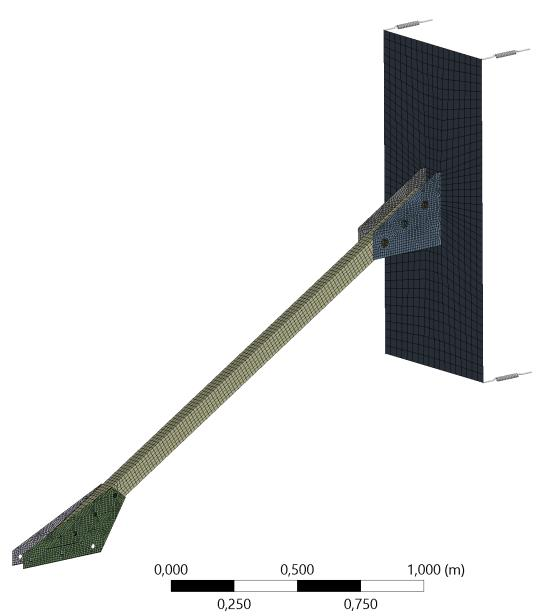
\includegraphics[width = \textwidth]{simsat-handle-model} 
		\caption{Конечно-элементная сетка} \label{subfig:simsat-handle-model}
	\end{subfigure}
	\hfill
	\begin{subfigure}[t]{0.49\textwidth}
		\centering
		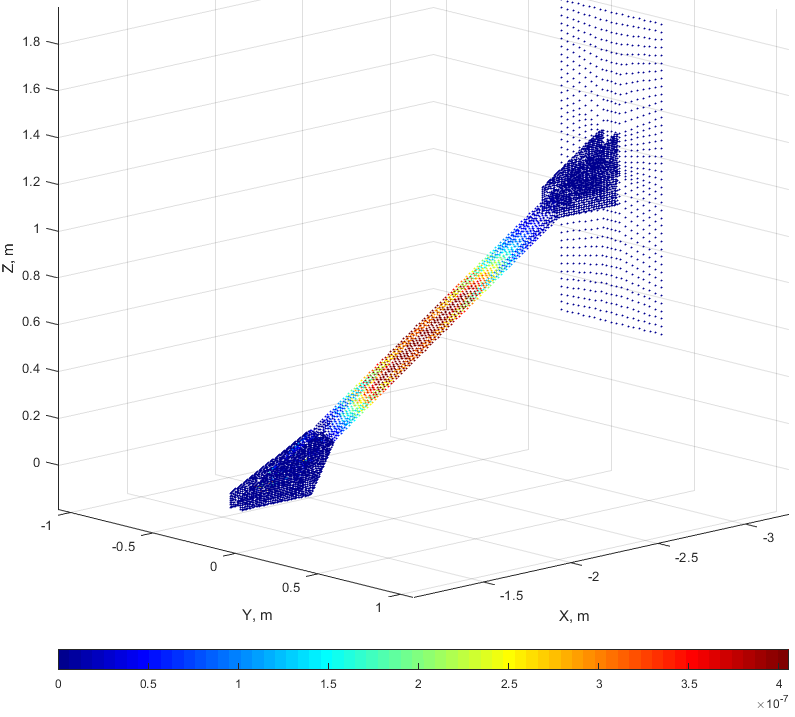
\includegraphics[width = \textwidth]{simsat-handle-coeffs}
		\caption{Распределение корректирующих жесткостей по узлам} \label{subfig:simsat-handle-coefs}
	\end{subfigure}	
	\caption{КЭ-модель штанги с <<упругой заделкой>>} 
\end{figure}

Скорректированная модель зонтичного каркаса освобождена от закрепления по методу, представленному в разделе~\ref{struct:freeing}. Формирование глобальной модели конструкции было проведено путем ассемблирования КЭ-моделей подконструкций по степеням свободы узлов стыковки по принципу формирования глобальной матрицы жесткости в методу конечных элементов.

Также, используя соотношения \eqref{eq:reducedGenParametersUpdating} и \eqref{eq:reducedStructuralMatrices}, была проведена коррекция редуцированных моделей штанги и зонтичного каркаса с последующим ассемблированием. Результаты сведены в таблице~\ref{tab:simsat-combined-results}. 

\begin{longtblr}[
	caption = {Результаты коррекции, освобождения и ассемблирования составных частей имитационной модели}, 
	label = {tab:simsat-combined-results}
]{
	colspec = {|X[c, -1]|X[c]|X[c]|X[c]|X[c]|X[c]|X[c]|}, 
	width = \textwidth, 
	rows = {font = \footnotesize},
	hline{5-12} = {solid}
}
	\hline	
	\SetCell[r = 3]{c} № & \SetCell[c = 6]{c} {Частоты собственных колебаний полной конструкции, Гц \\ (погрешность относительно эксперимента, \%)} \\ \cline{2-7}
	& \SetCell[r = 2]{c} Эксперимент & \SetCell[c = 2]{c} До коррекции && \SetCell[c = 3]{c} После коррекции \\ \cline{3-7}
	&& <<Идеальная заделка>> & <<Упругая заделка>> & Коррекция штанги & Коррекция штанги и антенны & Коррекция редуцированной штанги \\ \hline \hline
	1 & 1.726 & 1.852 (7.27\,\%) & 1.758 (1.84\,\%) & 1.738 (0.70\,\%) & 1.738 (0.70\,\%) & 1.758 (0.66\,\%) \\ 
    2 & 2.248 & 2.383 (6.01\,\%) & 2.335 (3.88\,\%) & 2.241 (0.33\,\%) & 2.239 (0.40\,\%) & 2.335 (2.76\,\%) \\ 
    3 & 5.215 & 5.430 (4.12\,\%) & 5.382 (3.19\,\%) & 5.280 (1.24\,\%) & 5.280 (1.24\,\%) & 5.382 (2.97\,\%) \\ 
    4 & 9.253 & 9.708 (4.92\,\%) & 9.450 (2.13\,\%) & 9.364 (1.18\,\%) & 9.364 (1.18\,\%) & 9.450 (1.78\,\%) \\ 
    5 & 11.98 & 12.44 (3.83\,\%) & 12.25 (2.25\,\%) & 12.32 (2.73\,\%) & 12.22 (1.95\,\%) & 12.25 (1.95\,\%) \\ 
    6 & 26.79 & 27.76 (3.64\,\%) & 27.74 (3.55\,\%) & 27.76 (3.48\,\%) & 27.74 (3.41\,\%) & 27.74 (3.45\,\%) \\ 
    7 & 27.22 & 28.25 (3.78\,\%) & 28.25 (3.78\,\%) & 28.25 (3.64\,\%) & 28.25 (3.64\,\%) & 28.25 (3.64\,\%) 
\end{longtblr}

Из таблицы~\ref{tab:simsat-combined-results} видно, что коррекция моделей составных частей приводит к удовлетворительному совпадению частот ассемблированной модели с соответствующими экспериментальными частотами. Важно отметить, что при коррекции моделей составных частей целевые значения частот были достигнуты с высокой точностью. Кроме того, при коррекции и создании матрицы демпфирования по результатам эксперимента методом \eqref{eq:finalObjFunUpdating} и по формулам \eqref{eq:reducedStructuralMatrices}, \eqref{eq:reducedDampingMatrix} амплитудно-частотные характеристики в окрестности резонансных частот практически совпадают.

На рисунке~\ref{subfig:simsat-mac-absolute} показаны изменения MAC-критерия до и после коррекции четырех низших частот, а на рисунке~\ref{subfig:simsat-mac-relative}~---~значения критерия модального соответствия между исходной и скорректированной моделью. Из рисунков видно, что в ходе коррекции происходит изменение форм собственных колебаний. Наиболее значительно изменилась вторая форма собственных колебаний, но величина этих изменений не превышает $ 0.14 $\,\% в метрике MAC-критерия.

\begin{figure}[H]
	\centering
	\begin{subfigure}[t]{0.49\textwidth}
		\centering
		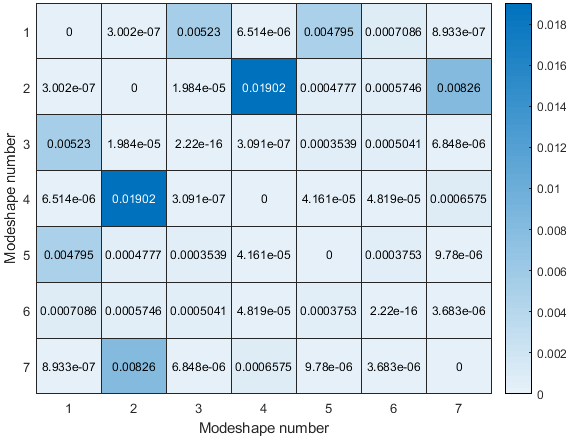
\includegraphics[width = \textwidth]{simsat-MAC-absolute}
		\caption{Изменение MAC-критерия по абсолютному значению} \label{subfig:simsat-mac-absolute}
	\end{subfigure}
	\hfill
	\begin{subfigure}[t]{0.47\textwidth}
		\centering
		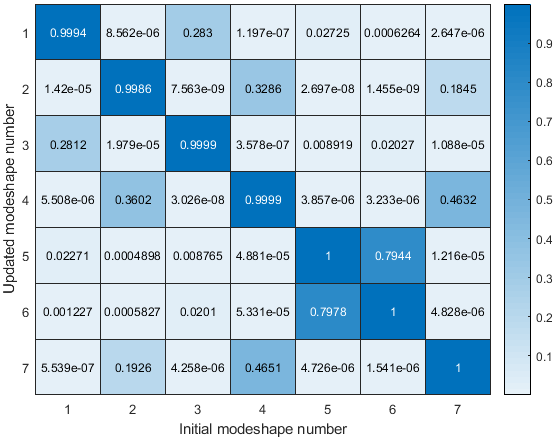
\includegraphics[width = \textwidth]{simsat-MAC-relative}
		\caption{MAC-критерий между исходной и скорректированной моделью} \label{subfig:simsat-mac-relative}
	\end{subfigure}	
	\caption{Оценка связи между формами собственных колебаний до и после коррекции} 
\end{figure}

В таблице~\ref{tab:simsat-full-results} представлены погрешности в определении частот собственных колебаний полноразмерной конструкции после коррекции, освобождения и синтеза моделей составных частей. 

\begin{longtblr}[
	caption = {Результаты полноразмерной коррекции, освобождения и ассемблирования при различном числе корректируемых тонов колебаний}, 
	label = {tab:simsat-full-results}
]{
	colspec = {|X[c, 1.4]|X[c]|X[c]|X[c]|X[c]|X[c]|X[c]|X[c]|X[c]|X[c]|}, 
	width = \textwidth,
	hlines
}
	{Номера \\ тонов} & \SetCell[c = 9]{c} {Погрешности частот скорректированной ассемблированной \\ модели по сравнению с частотами из эксперимента, \%} \\
	Штанги & 1 & 1,\,2 & 1\,--\,3 & 1\,--\,4 & 1\,--\,3 & 1\,--\,3 & 1\,--\,3 & 1\,--\,3 & 1\,--\,4 \\
	Антенны & \SetCell[c = 4]{c} --- &&& & 1 & 1,\,2 & 1,\,15 & 1,\,2,\,15 & 1,\,15 \\ \hline
	1 & -0.90 & -0.90 & 0.70 & 0.70 & 0.70 & 0.70 & 0.70 & 0.70 & 0.70 \\
	2 & 1.16 & 1.47 & 1.47 & -0.33 & 1.41 & 1.43 & 1.39 & 1.40 & -0.40 \\
	3 & 1.50 & 1.50 & 1.24 & 1.24 & 1.23 & 1.21 & 1.23 & 1.21 & 1.24 \\
	4 & 1.40 & 1.40 & 1.18 & 1.18 & 1.18 & 1.17 & 1.18 & 1.17 & 1.18 \\
	5 & 1.44 & 1.49 & 1.49 & 2.73 & 0.91 & 1.16 & 0.71 & 0.78 & 1.95 \\ 
	6 & 3.29 & 3.29 & 3.29 & 3.48 & 3.22 & 3.22 & 3.21 & 3.21 & 3.41 \\ 
	7 & 3.64 & 3.64 & 3.64 & 3.64 & 3.64 & 3.64 & 3.64 & 3.64 & 3.64 \\ 
\end{longtblr}

Можно видеть, что наибольшее влияние на частоты ассемблированной модели оказывает коррекция штанги, в то время как коррекция зонтичного каркаса приводит лишь к небольшому снижению результирующих погрешностей.

\section{Коррекция расчетной модели отъемной части крыла изделия \mbox{С-70}}

В настоящем разделе рассматривается применение метода коррекции к композитной отъемной части крыла (ОЧК) изделия \mbox{С-70}. 

\subsection{Экспериментальный модальный анализ}

Для проведения экспериментального модального анализа консоль крыла была вывешена вертикально на авиационных амортизационных шнурах посредством траверсы \figref{fig:wing-experiment}. Шнуры продевались через установленные в проушины узлов крепления технологические такелажные приспособления. Испытания выполнялись в соответствии методическими рекомендациями \cite{lib:aprobation:Moskalik}. 

\begin{figure}[H]
	\centerfloat
	\includegraphics[width = 0.7\linewidth]{wing-experiment}
	\caption{Общий вид ОЧК изделия \mbox{С-70} на упругой подвеске} \label{fig:wing-experiment}
\end{figure}

\subsection{Построение конечно-элементной модели}

В соответствии с исходными данными, переданными специалистами конструкторского бюро, конструктивно-силовой набор крыла представлялся невесомыми балочными и оболочечными элементами. Последние имеют характеристики обшивки и работают только на растяжение-сжатие, в то время как балочные элементы, лежащие в плоскости симметрии крыла, работают только на изгиб. При этом инерционные характеристик крыла воспроизводятся дискретными массами, имеющими эксцентриситет.

Для формирования геометрической модели использовались таблицы с координатами вершин поверхностей и концевых точек балок. Толщины элементов обшивки задавались дискретно по вершинам, образующим граничные поверхности. Распределение изгибных жесткостей внутри каждой балки описывалось полиномом третьей степени, заданным в равноотстоящих узлах. 

По результатам построения геометрической модели были замечено, что между некоторыми панельными элементами имеются существенные зазоры по высоте~---~нарушена непрерывность геометрического контура. Для обеспечения совместности перемещений элементов составлялись пары контактирующих ребер, которые примыкают друг к другу плоскости симметрии крыла. Кроме того, балочный каркас был спроецирован на обшивку для формирования линий контактного взаимодействия \figref{wing-intersection-isometric}. Массы размещались на ближайших точках балочного каркаса. При этом компоненты тензора инерции пересчитывались пропорционально относительному удалению массы от точки размещения. 

\begin{figure}[!htb]
	\centerfloat
	\includegraphics[width = \linewidth]{wing-intersection-isometric}
	\caption{Проецирование балочного каркаса и масс на элементы силового набора ОЧК} \label{wing-intersection-isometric}
\end{figure}

Посредством системы макросов \name{Ansys Mechanical APDL} была создана программа, позволяющая автоматически формировать конечно-элементную модель при изменении исходных данных. Геометрические модели балочного каркаса и обшивки приведены на рисунках~\ref{fig:wing-geometry-beams} и \ref{fig:wing-geometry-panels} соответственно. Число степеней свободы в модели составило $ 19710 $. Для сшивки панелей как между собой, так и с балочным каркасом, использовались абсолютно жесткие балки. Результирующая конечно-элементная модель приведена на рисунке~\ref{fig:wing-mesh}. Упругие формы собственных колебаний срединной поверхности модели приведены на рисунке~\ref{fig:wing-initial-mode}. Здесь и далее нумерация тонов колебаний начинается с первого тона упругих колебаний. 

\begin{figure}[!htb]
	\centerfloat
	\includegraphics[width = 0.85\linewidth]{wing-geometry-beams}
	\caption{Геометрическая модель балочного каркаса}\label{fig:wing-geometry-beams}
\end{figure}

\begin{figure}[!htb]
	\centerfloat
	\includegraphics[width = 0.85\linewidth]{wing-geometry-panels}
	\caption{Геометрическая модель обшивки}\label{fig:wing-geometry-panels}
\end{figure}

\begin{figure}[H]
	\centerfloat
	\includegraphics[width = 0.85\linewidth]{wing-mesh}
	\caption{Конечно-элементная модель ОЧК} \label{fig:wing-mesh}
\end{figure}

\def\sfWing{0.48\textwidth}

\begin{figure}[!htb]
	\centering
	\begin{subfigure}[t]{\sfWing}
		\centering
		\includegraphics[width = \textwidth]{wing-initial-mode-1}
	\end{subfigure}
	\hfill
	\begin{subfigure}[t]{\sfWing}
		\centering
		\includegraphics[width = \textwidth]{wing-initial-mode-2}
	\end{subfigure}	
	\begin{subfigure}[t]{\sfWing}
		\centering
		\includegraphics[width = \textwidth]{wing-initial-mode-3}
	\end{subfigure}	
	\hfill
	\begin{subfigure}[t]{\sfWing}
		\centering
		\includegraphics[width = \textwidth]{wing-initial-mode-4}
	\end{subfigure}	
	\caption{Пример упругих форм колебаний исходной КЭ-модели ОЧК} \label{fig:wing-initial-mode}
\end{figure}

\subsection{Коррекция конечно-элементной модели}

Коррекция КЭ-модели проводилась по пяти наборам экспериментально определенных частот. Каждый последующий набор дополнял предыдущий одним тоном колебаний. Так, cначала была проведена коррекция только по изгибу ОЧК I тона, а затем еще и по изгибу ОЧК II тона. В конечном итоге была осуществлена одновременная коррекция 5 тонов колебаний \tabref{tab:wing-results}. 

\begin{longtblr}[
	caption = {Результаты коррекции ОЧК}, 
	label = {tab:wing-results}
]{
	colspec = {|c|c|c|X[c]|X[c]|X[c]|X[c]|X[c]|X[c]|}, 
	width = \textwidth, 
	hlines
}
	\SetCell[r = 3]{c} Тон & \SetCell[c = 2]{c} Приведенная частота && \SetCell[c = 6]{c} Погрешность до и после коррекции, \% \\
	& \SetCell[r = 2]{c} Эксперимент & \SetCell[r = 2]{c} {Исходная \\ модель} & \SetCell[r = 2]{c} До & \SetCell[c = 5]{c}После \\
	& & & & 1 & 2 & 3 & 4 & 5 \\ \hline
	1 & 1.00 & 1.51 & 50.7 & 0.0 & 0.0 & 0.0 & 0.0 & 0.0 \\ 
	2 & 2.28 & 3.18 & 39.5 & -7.4 & 0.0 & 0.0 & 0.0 & 0.0 \\ 
	3 & 3.37 & 4.13 & 22.6 & -18.6 & -13.8 & 0.0 & 0.0 & 0.0 \\ 
	4 & 3.95 & 4.82 & 21.8 & -19.1 & -17.8 & -8.2 & 0.0 & 0.0 \\ 
	5 & 4.87 & 6.15 & 26.2 & -16.2 & -21.8 & -2.6 & -4.4 & 0.0 \\ 
\end{longtblr}

Распределения изменений узловых жестокостей по всем линейным степеням свободы КЭ-модели до и после коррекции по первому тону и пяти тонам колебаний приведены на рисунках~\ref{subfig:wing-coeffs-1} и \ref{subfig:wing-coeffs-5} соответственно. Необходимо отметить, что изменения узловых жесткостей при коррекции по пяти тонам посчитаны относительно жесткостей, полученных в результате коррекции по первому тону. Синяя цветовая гамма на рисунках соответствует областям понижения исходной жесткости, а красная~---~областям повышения исходной жесткости. Черному цвету соответствуют области, жесткость которых в ходе коррекции осталась неизменной. 

\begin{figure}[!htb]
	\centering
	\begin{subfigure}[t]{\sfWing}
		\centering
		\includegraphics[width = \textwidth]{wing-coeffs-1}
		\caption{По одному тону} \label{subfig:wing-coeffs-1} 
	\end{subfigure}
	\hfill
	\begin{subfigure}[t]{\sfWing}
		\centering
		\includegraphics[width = \textwidth]{wing-coeffs-5}
		\caption{По пяти тонам} \label{subfig:wing-coeffs-5}
	\end{subfigure}	
	\caption{Распределения изменений узловых жестокостей по всем линейным степеням свободы КЭ-модели до и после коррекции}
\end{figure}

Вследствие изменения упругости корректируемой модели происходит изменение частот и форм колебаний. Нормированные к массе формы колебаний срединной поверхности модели до (черным цветом) и после коррекции (красным цветом) по пяти частотам собственных колебаний приведены на рисунках~\ref{subfig:wing-compare-mode-1}~--~\ref{subfig:wing-compare-mode-5}.

\begin{figure}[!htb]
	\centering
	\begin{subfigure}[t]{\sfWing}
		\centering
		\includegraphics[width = \textwidth]{wing-compare-mode-1}
		\caption{} \label{subfig:wing-compare-mode-1} 
	\end{subfigure}
	\hfill
	\begin{subfigure}[t]{\sfWing}
		\centering
		\includegraphics[width = \textwidth]{wing-compare-mode-2}
		\caption{} 
	\end{subfigure}	
	\begin{subfigure}[t]{\sfWing}
		\centering
		\includegraphics[width = \textwidth]{wing-compare-mode-3}
		\caption{} 
	\end{subfigure}	
	\hfill
	\begin{subfigure}[t]{\sfWing}
		\centering
		\includegraphics[width = \textwidth]{wing-compare-mode-4}
		\caption{} 
	\end{subfigure}	
	\begin{subfigure}[t]{\sfWing}
		\centering
		\includegraphics[width = \textwidth]{wing-compare-mode-5}
		\caption{} \label{subfig:wing-compare-mode-5} 
	\end{subfigure}	
	\caption{Сопоставление первых пяти упругих форм колебаний ОЧК до и после коррекции~(а~--~д)}
\end{figure}

Таблица соответствия форм колебаний до и после коррекции по критерию модального соответствия приведена на рисунке~\ref{fig:wing-mac}. Из рисунка видно, что формы колебаний до и после коррекции удовлетворительно коррелируют между собой.

\begin{figure}[H]
	\centerfloat
	\includegraphics[width = 0.7\linewidth]{wing-mac}
	\caption{Таблица соответствия форм колебаний до и после коррекции} \label{fig:wing-mac}
\end{figure}

\section{Коррекция расчетной модели гирдера для модульных секций накопителя ЦКП <<СКИФ>>}

Центр коллективного пользования <<Сибирский кольцевой источник фотонов>> (ЦКП~<<СКИФ>>) можно условно представить в виде инжекционной части, состоящей из бустерного синхротрона и линейного ускорителя, и накопительного кольца. В первой части происходит создание электронного пучка, обладающего требуемой энергией, который затем преобразуется и накапливается в виде синхротронного излучения в накопительной части. Ключевым требованием к последней является обеспечение максимальной продолжительности жизни пучка и сохранение его интенсивности. Среди прочего, это достигается за счет прецизионного выставления многочисленного электрофизического оборудования на специальных подставках, именуемых гирдерами. К посадочным поверхностям последних предъявляются высокие требования по точности размещения и регулирования. Более того, во избежание возникновения резонансов, приводящих к потере качества пучка, собственные частоты гирдера должны быть отстроены от парциальных частот оборудования и сейсмических колебаний. Решение этой задачи реализуется в три этапа: проектирование, производство и экспериментальная отработка гирдера. Для обоснования и проработки конструкторских решений на первом этапе использовался метод конечных элементов.

В соответствии с конструкторской документаций была построена геометрическая модель гирдера накопительного кольца~\figref{fig:girder-geometry} длиной $ 3800 $ мм (\name{G3800}). Масса гирдера составила $ 2166 $ кг. 

\begin{figure}[H]
	\centering
	\includegraphics[width = 0.6\linewidth]{girder-geometry}
	\caption{Геометрическая модель гирдера} \label{fig:girder-geometry}
\end{figure}

Конструктивное исполнение регулируемых опор гирдера раскрыто на рисунках~\ref{fig:girder-supports} и \ref{fig:girder-support-section}. Особо отметим, что низшие частоты собственных колебаний гирдера в значительной степени обусловлены динамической жесткостью опор.

\begin{figure}[!htb]
	\centering
	\includegraphics[width = 0.7\linewidth]{girder-supports}
	\caption{Регулируемые опоры гирдера} \label{fig:girder-supports}
\end{figure}

\begin{figure}[!htb]
	\centering
	\includegraphics[width = 0.4\linewidth]{girder-support-section}
	\caption{Сечение регулируемой опоры гирдера} \label{fig:girder-support-section}
\end{figure}

Для определения совместного отклика модульной секции магниты размещались на поверхности гирдера согласно рабочей документации института ядерной физики имени Г\,.\,И.~Будкера~СО~РАН \figref{fig:girder-full-system}.

\begin{figure}[!htb]
	\centering
	\includegraphics[width = 0.7\linewidth]{girder-full-system}
	\caption{Совместная геометрическая модель гирдера и магнитов} \label{fig:girder-full-system}
\end{figure}

Необходимо заметить, что крепежные элементы, составные части системы охлаждения совместной системы гирдера и магнитов не оказывают существенного влияния на определяемые статические и динамические характеристики, поэтому геометрическая модель рассматриваемой системы была упрощена. Общие упрощения, использованные при построении конечно-элементных моделей магнитов:
\begin{itemize}
	\item крепежные элементы, не относящиеся к опорам, исключены и заменены контактными элементами;
	\item отверстия, соответствующие отброшенным крепежным элементам, заполнены материалом;
	\item распределение материала по каждому из магнитов считалось изотропным;
	\item плотность материала каждого магнита подбиралась так, чтобы его масса соответствовала массе позиции на чертеже рабочей документации.
\end{itemize} 

Таким образом, была получена упрощенная геометрическая модель системы, на основе которой строилась конечно-элементная модель. Она использовалась для получения первичных оценок напряженно-деформированного состояния под воздействием весовых нагрузок и частот собственных колебаний. 

По результатам расчётов доработано расположение и конструктивное исполнение регулируемых опор. Изменены геометрические параметры фундаментных опор и балок. Конструкция дополнена плитой с целью повышения жесткости гирдера в поперечном направлении. На основании выработанных конструкторских решений гирдер был произведен и испытан средствами экспериментального модального анализа~\figref{fig:girder-experiment}.

\begin{figure}[H]
	\centering
	\includegraphics[width = 0.75\linewidth]{girder-experiment}
	\caption{Модальные испытания гирдера без магнитов} \label{fig:girder-experiment}
\end{figure}

По результатам экспериментальных исследований было установлено, что формы собственных колебаний, соответствующие низшим тонам, происходят при совместном перемещении гирдера и блока фундамента, на который опираются регулируемые опоры~\figref{fig:girder-spring-mode}.

\begin{figure}[!htb]
	\centering
	\includegraphics[width = 0.6\linewidth]{girder-spring-mode}
	\caption{Пример формы колебаний гирдера на упругом основании} \label{fig:girder-spring-mode}
\end{figure} 

Такое упругое поведение фундамента существенно отличается от модели жесткого закрепления, использованной в предварительных расчетах. Было принято решение построить модель упругого основания~\figref{fig:girder-mesh}, используя пружины, жесткости которых определялись автоматически по результатам решения задачи коррекции для первых пяти частот собственных колебаний, отвечающих этим движениям. Целевые значения частот достигнуты со степенью точности $ 2 \cdot 10 ^ {-8} $ по критерию~\eqref{eq:convergenceCriterion}.

\begin{figure}[H]
	\centering
	\includegraphics[width = 0.55\linewidth]{girder-mesh}
	\caption{Конечно-элементная модель гирдера на упругом основании} \label{fig:girder-mesh}
\end{figure}

Полученная модель гирдера на фундаменте использовалась для осуществления одновременной коррекции по шести частотам упругих тонов собственных колебаний~\figref{fig:girder-elastic-mode}. Коррекция КЭ-модели производилась без удержания частот собственных колебаний, соответствующих движениям на упругом основании. Это объясняется отсутствием  экспериментальных данных о характере зависимости частот от уровня приложенных нагрузок. Целевые значения коррекции были достигнуты с высокой степенью точности~\tabref{tab:girder-results}.

\begin{figure}[!htb]
	\centering
	\includegraphics[width = 0.6\linewidth]{girder-elastic-mode}
	\caption{Пример упругой формы колебаний гирдера} \label{fig:girder-elastic-mode}
\end{figure}

\begin{longtblr}[
	caption = {Результаты коррекции гирдера}, 
	label = {tab:girder-results}
]{
	colspec = {|X[c, -1]|X[c]|X[c]|X[c]|X[c]|}, 
	width = \textwidth, 
	hlines
}
	\SetCell[r = 2]{c} Тон & \SetCell[c = 2]{c} Частота, Гц && \SetCell[c = 2]{c} Погрешность, \% \\
	& Эксперимент & Исходная модель & До коррекции & После коррекции \\ \hline
	6 & 119.51 & 135.08 & 13.03 & \SetCell[r = 6]{c} \textbf{0.00} \\
	7 & 140.97 & 146.46 & 3.89 &  \\
	8 & 148.13 & 160.07 & 8.06 &  \\
	9 & 189.65 & 210.48 & 10.98 & \\
	10 & 197.53 & 214.18 & 8.43 & \\
	11 & 242.24 & 253.51 & 4.65 & \\
\end{longtblr}

Наибольшие изменения узловых жесткостей~\figref{fig:girder-coeffs} достигаются в местах сопряжения конструктивных элементов гирдера. Минимальный критерий модального соответствия, связывающий формы колебания до и после коррекции, составил $ 0.9412 $~\figref{fig:girder-mac}. Суммарные модальные эффективные массы~\cite{lib:modelUpdating:Ewins} корректируемых тонов колебаний по направлениям глобальной системы координат составили: $ 79 $, $ 96 $ и $ 97 $ \%. 

\def\sfGirder{0.48\textwidth}

\begin{figure}[!htb]
	\centering
	\begin{subfigure}[t]{\sfGirder}
		\centering
		\includegraphics[width = \textwidth]{girder-coeffs-0-6} 
		\caption{Относительно исходной модели} 
	\end{subfigure}
	\hfill
	\begin{subfigure}[t]{\sfGirder}
		\centering
		\includegraphics[width = \textwidth]{girder-coeffs-1-6}
		\caption{Относительно коррекции по одной частоте} 
	\end{subfigure}	
	\caption{Распределения изменений узловых жестокостей по всем линейным степеням свободы КЭ-модели до и после коррекции} \label{fig:girder-coeffs}
\end{figure}

\begin{figure}[!htb]
	\centering
	\includegraphics[width = 0.7\linewidth]{girder-mac}
	\caption{Таблица соответствия форм колебаний до и после коррекции} \label{fig:girder-mac}
\end{figure}

Для оценки эффективности разработанных вычислительных алгоритмов, приведем данные о продолжительности работы программы на каждом этапе коррекции:
\begin{enumerate}
	\item Уточнение упругих характеристик основания~---~$ 2 $~минуты.
	\item Коррекция четырех упругих тонов, происходящих при преимущественном движении в горизонтальной плоскости~---~$ 7 $~минут.
	\item Коррекция двух упругих тонов, происходящих при преимущественном движении в вертикальной плоскости~---~$ 1 $~минута.
	\item Коррекция всех шести упругих тонов~---~$ 4 $~минуты.
\end{enumerate}

Таким образом, длительность коррекции расчетной модели гирдера с числом степеней свободы~$ 304 $ тысячи составила $ 14 $~минут. Уточнение расчетной динамической модели позволит улучшить эксплуатационные характеристики совместной системы гирдера и магнитов.

\section{Выводы по главе \thechapter}

Разработанные методики использованы для решения практических задач коррекции, освобождения и синтеза расчетных динамических моделей конструкций. Получены следующие основные результаты:
\begin{enumerate}
	\item Осуществлена последовательная коррекция динамически-подобной модели самолёта Ту-204 по шести наборам экспериментально определенных частот собственных колебаний. Показано, что на каждом шаге коррекции, дополняющим предыдущий одним тоном колебаний, происходит уточнение расчетной модели.
	\item Выполнен синтез расчетных моделей составных частей модели каркаса зонтичной антенны. Податливость закрепления штанги учтена посредством подхода, состоящего в проведении дополнительных статических испытаний. Показано, что коррекция моделей составных частей приводит к уточнению частот собственных колебаний синтезированной модели.
	\item Проведен экспериментальный модальный анализ отъемной части крыла изделия С-70. По результатам испытаний выявлено, что полученные частоты собственных колебаний консоли крыла существенно отличаются от расчетных. Однако, в результате применения разработанной методики коррекции, целевые значения частот были достигнуты с заданной степенью точности. 
	\item Проведена двухэтапная коррекция КЭ-модели гирдера для модульных секция накопителя ЦКП <<СКИФ>>. На первом этапе проведено уточнение жесткостных характеристик основания по пяти частотам собственных колебаний, происходящих при совместном движении гирдера и фундамента. На следующем этапе, используя шесть экспериментально определенных частот, были успешно уточнены упругие характеристики гирдера. Показано, что формы собственных колебаний после коррекции остаются согласованными со своими исходными аналогами в смысле критерия модального соответствия.
\end{enumerate}

Основные результаты, изложенные в данной главе, опубликованы в работах~\cite{lib:author:chinese:updating, lib:author:iss2021:updating, lib:author:dvm:updating, lib:author:iss2022:updating}. Практическая значимость полученных результатов подтверждается актами об использовании и внедрении~(приложения~\ref{struct:acts-usage} и \ref{struct:acts-implement}).